%% Template.tex; Solar Physics
%% 
\documentclass[namedreferences]{solarphysics}
%
% spr-sola-addons available options:
%  hyperref      -- loads hyperref.sty with options (pdfborder={0 0 0 },urlcolor=blue,breaklinks)
%  nonatbib      -- do not load natbib.sty (style loads it by default)
%  solaromanenum -- makes enumerated list with roman numerals and a single right-bracket
%  linksfromyear -- puts a link on a year citation (hyperref must be loaded). Loaded by default
%  nolinksfromyear -- suppress  linksfromyear
%  optionalrh    -- for optional running title/author
%  showbiblabels -- to show bibitem label at end of bibitem (via \endbibitem command)
%
\usepackage[hyperref,optionalrh,solaromanenum]{spr-sola-addons} % For Solar Physics 
%\usepackage{epsfig}                     % For eps figures, old commands
\usepackage{graphicx}                    % For eps figures, newer & more powerfull
%\usepackage{courier}                    % Change the \texttt command to courier style
\usepackage{amssymb}                     % useful mathematical symbols
\usepackage{color}                       % For color text: \color command
\usepackage{breakurl}                    % For breaking URLs easily trough lines
\def\UrlFont{\sf}                        % define the fonts for the URLs
\usepackage{comment}
\usepackage{setspace}
\usepackage[utf8]{inputenc}
\usepackage[dvipsnames]{xcolor}

%% Local definitions
%% please place your own definitions here and don't use \def but
%% \newcommand{}{} or 
%% \renewcommand{}{} if it is already defined in LaTeX
\renewcommand{\deg}{$^\circ$}
\newcommand{\mdeg}{^\circ}
\newcommand{\rsun}{R{$_\odot$}}
\renewcommand{\l}{\lambda_{\rm N}}%\lambda_
\newcommand{\mrsun}{{\rm R_\odot}}
\newcommand{\med}{{\rm Md}}
\newcommand{\avgTe}{\left<\Tm\right>}
\newcommand{\MK}{{\rm MK}}
\newcommand{\cm}{{\rm cm}}
\newcommand{\sdev}{{\rm SD}}
\newcommand{\mean}{{\rm Mn}}
\newcommand{\deltat}{$\delta$}
\newcommand{\LDEM}{{\rm LDEM}}
\newcommand{\FBE}{{\rm FBE}}
\newcommand{\TRF}{{\rm TRF}}
\newcommand{\lN}{\lambda_N}
\newcommand{\NCB}{N_{\rm CB}}
\newcommand{\aTm}{\left< \Tm\right>}
\newcommand{\Nqi}{N_{\rm QI}}
\newcommand{\sqravgN}{\sqrt{\langle N_{e,i}^2 \rangle}}
\newcommand{\dr}{\triangledown_r}
\newcommand{\er}{\mathbf{e}_r}
\newcommand{\Te}{T_{\rm e}}
\newcommand{\Tm}{T_{\rm m}}
\newcommand{\Ne}{N_{\rm e}}
\newcommand{\rhoTr}{\rho(T,r)}
\newcommand{\Tefit}{T_{e,{\rm fit}}}

\newcommand{\BibTeX}{\textsc{Bib}\TeX}
\newcommand{\etal}{{\it et al.}}

\newcommand{\Pl}{\texttt{+}}
\newcommand{\Mi}{\texttt{-}}

% Definitions for the journal names
\newcommand{\adv}{    {\it Adv. Space Res.}} 
\newcommand{\annG}{   {\it Ann. Geophys.}} 
\newcommand{\aap}{    {\it Astron. Astrophys.}}
\newcommand{\aaps}{   {\it Astron. Astrophys. Suppl.}}
\newcommand{\aapr}{   {\it Astron. Astrophys. Rev.}}
\newcommand{\ag}{     {\it Ann. Geophys.}}
\newcommand{\aj}{     {\it Astron. J.}} 
\newcommand{\apj}{    {\it Astrophys. J.}}
\newcommand{\apjs}{   {\it Astrophys. J. Suppl.}}
\newcommand{\apjl}{   {\it Astrophys. J. Lett.}}
\newcommand{\apss}{   {\it Astrophys. Space Sci.}} 
\newcommand{\cjaa}{   {\it Chin. J. Astron. Astrophys.}} 
\newcommand{\gafd}{   {\it Geophys. Astrophys. Fluid Dyn.}}
\newcommand{\grl}{    {\it Geophys. Res. Lett.}}
\newcommand{\ijga}{   {\it Int. J. Geomagn. Aeron.}}
\newcommand{\jastp}{  {\it J. Atmos. Solar-Terr. Phys.}} 
\newcommand{\jgr}{    {\it J. Geophys. Res.}}
\newcommand{\mnras}{  {\it Mon. Not. Roy. Astron. Soc.}}
\newcommand{\nat}{    {\it Nature}}
\newcommand{\pasp}{   {\it Pub. Astron. Soc. Pac.}}
\newcommand{\pasj}{   {\it Pub. Astron. Soc. Japan}}
\newcommand{\pre}{    {\it Phys. Rev. E}}
\newcommand{\solphys}{{\it Solar Phys.}}
\newcommand{\sovast}{ {\it Soviet  Astron.}} 
\newcommand{\ssr}{    {\it Space Sci. Rev.}} 

%%%%%%%%%%%%%%%%%%%%%%%%%%%%%%%%%%%% temporales
\definecolor{mygray}{gray}{0.6}


%---------REMOVE DEFs BEFORE SUMBISSION----------------
\def\diego#1{\textcolor{red}{DIEGO: #1}}
\def\albert#1{\textcolor{blue}{#1}}
\def\fede#1{\textcolor{ForestGreen}{FEDE: #1}}
\def\temp#1{\textcolor{mygray}{#1}}
\def\edit#1{\textcolor{Apricot}{#1}}
%------------------------------------------------------


%%%%%%%%%%%%%%%%%%%%%%%%%%%%%%%%%%%%%%%%%%%%%%%%%%%%%%%%%%%%%%%%%%
\begin{document}

\begin{article}

\begin{opening}

\title{Thermodynamic Structure of the Solar Corona: Tomographic Reconstructions and MHD Modeling}

%%%%%%%%%%%%%%%%%%%%%%%%%%%%%%%%%%%%%%%%%%%%%%%%%%%
%% Authors Names
%
% \author[addressref={},corref,email={}]{\inits{}\fnm{}\lnm{}\orcid{}}
\author[addressref={aff1},corref,email={dlloveras@iafe.uba.ar}]{\inits{D.G.}\fnm{Diego G.}~\lnm{Lloveras}\orcid{0000-0003-1402-0398}}

\author[addressref={aff1,aff3},corref,email={albert@iafe.uba.ar}]{\inits{A.M.}\fnm{Alberto M.}~\lnm{V\'asquez}\orcid{0000-0003-3401-6409}} 

\author[addressref={aff1},corref,email={federico@iafe.uba.ar}]{\inits{F.A.}\fnm{Federico A.}~\lnm{Nuevo}\orcid{0000-0003-2355-5853}} 

\author[addressref={aff1,aff3},corref,email={cmaccormack@iafe.uba.ar}]{\inits{C.}\fnm{Cecilia}~\lnm{Mac Cormack}}

\author[addressref={aff4},corref,email={nishthas@umich.edu}]{\inits{N.}\fnm{Nishtha}~\lnm{Sachdeva}\orcid{1}}

\author[addressref={aff4},corref,email={chipm@umich.edu}]{\inits{W.}\fnm{Ward}~\lnm{Manchester IV}\orcid{2}}

\author[addressref={aff4},corref,email={bartvand@umich.edu}]{\inits{B.}\fnm{Bartholomeus}~\lnm{Van der Holst}\orcid{3}}

\author[addressref={aff4},corref,email={rfrazin@umich.edu}]{\inits{R.A.}\fnm{Richard A.}~\lnm{Frazin}\orcid{0000-0002-0281-7677}}

%%%%%%%%%%%%%%%%%%%%%%%%%%%%%%%%%%%%%%%%%%%%%%%%%%%
%% Runningheads
%
\runningauthor{D.G.~Lloveras~\etal}
%\runningtitle{}


%%%%%%%%%%%%%%%%%%%%%%%%%%%%%%%%%%%%%%%%%%%%%%%%%%%
%% Affilations 
%% id shold be the same with \author addressref value.
%\address[id={}]{}
\address[id=aff1]{Instituto de Astronom\'{\i}a y F\'{\i}sica del Espacio (IAFE), CONICET-UBA, CC 67 - Suc 28,  (C1428ZAA) Ciudad Aut\'onoma de Buenos Aires, Argentina}

%\address[id=aff2]{Departamento de F\'{\i}sica, Facultad de Ciencias Exactas y Naturales (FCEN), Universidad de Buenos Aires (UBA), Pabell\'on I, Ciudad Universitaria, (C1428ZAA) Ciudad Aut\'onoma de Buenos Aires, Argentina}

\address[id=aff3]{Departamento de Ciencia y Tecnolog\'{\i}a, Universidad Nacional de Tres de Febrero (UNTREF), Valent\'{\i}n G\'omez 4752, (B1678ABH) Caseros, Provincia de Buenos Aires, Argentina}

\address[id=aff4]{Department of Climate and Space Sciences and Engineering (CLaSP), University of Michigan, 2455 Hayward Street, Ann Arbor, MI 48109-2143, USA}
%%%%%%%%%%%%%%%%%%%%%%%%%%%%%%%%%%%%%%%%%%%%%%%%%%%
%%% Abstract 
\begin{abstract}
Observational \albert{techniques} play an essential role in advancing our understanding of the physics of the solar corona. They provide validation data to improve three-dimensional (3D) magnetohydrodynamic (MHD) models of the solar atmosphere, \albert{enhancing} their space weather forecasting capabilities. Solar rotational tomography (SRT) is currently the sole observational technique that provides an empirical 3D description of some \albert{of the fundamental} plasma parameters of the solar corona at a global scale. Based on EUV data of space borne instruments, SRT allows constructing 3D maps of the coronal electron density and temperature at heliocentric heights below 1.25 Rsun. We carry out a study of the corona combining tomographic reconstructions with MHD simulations \albert{using} the latest version of the Alfv\'en Wave Solar Model (AWSoM) of the Space Weather Modeling Framework (SWMF). Target rotations were selected from the solar minimum between solar cycles (SC) 23 and 24 and the current declining phase of solar cycle 24. Tomographic reconstructions and results of the model are analyzed in distinct coronal magnetic structures. We study magnetically closed structures associated with the equatorial streamer belt, as well as magnetically open regions enclosing it. We report on the tomographic results in the different structures, their implications for the physics of the solar corona, and the capability of the AWSoM model to reproduce the tomographic reconstructions in different regions.

\end{abstract}



%%%%%%%%%%%%%%%%%%%%%%%%%%%%%%%%%%%%%%%%%%%%%%%%%%%
%% Keywords
%
\keywords{Solar Cycle, Observations; Corona,E; Corona, Structures}


\end{opening}
%-------------------------------------------------

%%%%%%%%%%%%%%%%%%%%%%%%%%%%%%%%%%%%%%%%%%%%%%%%%%%
%% Sections
\section{Introduction}\label{intro} 

Being the place where the solar atmosphere is heated and the solar wind accelerated, and where impulsive events such as solar flares and coronal mass ejections are energized, observation and modeling of the solar corona are tasks of great relevance to improve our understanding of the Sun-Earth environment. To advance our knowledge of the physics of the solar corona, as well as to improve its three-dimensional (3D) models, information derived from observational data plays a key role. Solar rotational tomography is currently the sole observational technique able to provide a quantitative empirical description of the 3D distribution of some fundamental plasma parameters of the solar corona at a global scale.


\section{Methodology}\label{meto}   

\subsection{DEMT reconstructions}\label{demt}
\temp{* Procesado de imagenes}\\
\temp{* FBE}\\
\temp{* LDEM}\\
*Paso 1: obtencion de FBE\\
*Paso 2: obtencion LDEM
\begin{equation}\label{fbeldem}
\FBE_i^{(k)}  = \int\,\textrm{d}T\,\LDEM_i(T)\,{\TRF}^{(k)}(T), \ \ \ {k=1,...,K}
\end{equation}

\temp{
Due to unresolved coronal dynamics, tomographic reconstructions exhibit negative values of the reconstructed FBE, or zero when the solution is constrained to positive values \citep{frazin_2000,frazin_2009}. These non-reconstructed voxels are indicated as black voxels in the Carrington maps of the reconstructed DEMT reults in Section \ref{resu}.
}

Once the LDEM is determined at each voxel, the average squared electron density $\langle \Ne^2 \rangle$ and the electron mean temperature $\Tm$ in the voxel can be computed by taking its zeroth and first moments over temperature. More specifically, at the $i$-th voxel,

\begin{eqnarray}\label{momento1}
\langle N_{e,i}^2 \rangle &=& \int\,\textrm{d}T\,\LDEM_i(T),\label{Ne} \\ 
\label{momento2}
 T_{\textrm{m},i}   &=& \frac{1}{\langle N_{e,i}^2 \rangle}\,\int\,\textrm{d}T\,T\,\LDEM_i(T),\label{Tm} 
\end{eqnarray}


\albert{We define next a measure of the average relative difference between the tomographic and the synthetic FBE in each voxel, as}

\begin{equation}\label{R}
R_i \, \equiv \ (1/K) \, \sum_{k=1}^K \left| \, 1 - \FBE^{(k)}_{i,\rm syn}\,/\,\FBE^{(k)}_{i,\rm tom}\, \right| \,,
\end{equation}

so that the final product of DEMT is in the form of 3D maps of the electron density and mean temperature. These relationships \albert{were} derived in detail in \citealt{frazin_2009} (see Appendix C).\\
\temp{* Aclarar que consideramos Ne como $\sqrt{<\Ne ^2>}$.} \albert{ALBERT: Yo creo que es mejor simplemente hablar de $\sqravgN$}\\
\temp{* Mejoras de la DEMT con respecto a trabajos previos}.

\temp{DEMT has been improved since the previously published work. We now perform hollow-tomography with the EUV images, (definir hollow-tom) and a 3D regularized of the solution was applyed to obtain smother and more reliable result at the edge of the tomographic grid.}

\subsection{AWSoM simulations}\label{awsom} 
\temp{* Qué es, qué modela, qué datos usa, y qué se obtiene en general y en particular para este trabajo}\\
\temp{* Se debe aclarar que solo produce resultados razonables arriba de 1.065}\\
\temp{No pondría los mapas de 1.025 y diria algo asi como:}\\
In the transition region \albert{(TR)}, the plasma heats up and becomes less dense \albert{by} several orders of magnitude \albert{over} a short distance. Modeling this region \albert{realistically has a very high computational cost}. For this \albert{reason,} the model uses \albert{an artificially} extended \albert{TR about $\approx 0.05\,\mrsun$ thick, as well as artificially high boundary conditions for the electronic density and temperature}. Consequently, model results below \albert{$\approx 1.05\,\mrsun$} were not taken into account in this article.

\subsection{Tracing results along fieldlines}\label{trace} 

\diego{Falta explicar que todos los resultados pasamos a tenerlos en la grilla demt, y que en esa grilla se traza el campo.}

For both rotations, the DEMT and AWSoM 3D maps of electron density $\Ne$, electron mean temperature $\Tm$ and electron temperature $\Te$ respectively were traced along the magnetic field lines modeled using AWSoM as described at the end of Section \ref{demt}. In the case of closed loops, results were separated into their two legs, defined as the two segments that go from the coronal base up to the apex.

For each open field line, and for each leg of the closed ones, an exponential fit was then applied to the $\Ne(r)$ data points, and a linear fit applied to the $\Tm(r)$ data points, as described by

\begin{eqnarray}\label{Nfit}
\Ne &=& N_0\,\exp{\left[\,-\,\left(h/\l\right)\,/\,\left(r/\mrsun\right)\,\right]}\\
\label{Tfit}
\albert{\Tm} &=& \albert{\dr \Tm(r) \ r\,+\,T_0}
\end{eqnarray}
 
\noindent
\albert{where $\l$ is the electron density scale height, $h \equiv r - 1\,\mrsun$ is the coronal height measured from the photosphere, $\dr\equiv\er\cdot\nabla$ is the radial derivative operator (being $\er$ the heliocentric radial unit vector), and $T_0$ and $N_0$ are constants.}

In the case of the electron density, the fitted function corresponds to the isothermal hydrostatic equilibrium solution, allowing for variation of the solar gravitational acceleration with height. After computing the footpoint ($r=1.0\,\mrsun$) electron density $N_{0}\,[\cm^{-3}]$ and scale height $\lN\,[\mrsun]$\temp{, this choice of function provides a straightforward means to directly evaluate how compatible is the observed coronal thermodynamical state with the hydrostatic solution}.

%La temperatura en funcion de la altura a lo largo de lineas muestra comportamientos lineales. En el presente trabajo nos focalizamos en lineas con temperaturas crecientes y decrecientes en foma lineal. Es decir nos quedamos con aquellas piernas donde el coeficiente de pearson entre la temperatura y la altura (rho) cumple rho mayor 0.5 (con p-value 0.05) y de esta forma se descartan aquellas piernas en las que los resultados DEMT no pueden asegurar un cambio notable de temperatura entre la base y el apice (asi no uso la palabra isotermico y evado ese problema)


%The temperature as a function of height along legs shows linear behaviors. 
In the present work we focus on lines with increasing and decreasing temperatures in linear form. In other words, we selected those legs where the \albert{Pearson correlation coefficient $\rho$ between temperature $T$ and radius $r$ meets $|\rhoTr| > 0.5$}. \temp{(with p-value less than 0.05)}. In this way, those legs in which the DEMT results cannot ensure a noticeable change in temperature between the base and the apex, are discarded.


The linear fit allows characterization of its variation with height by means of a characteristic temperature gradient $\dr \Tm\,[\MK/\mrsun]$ along each leg.
\diego{En realidad esta regresion lineal utiliza de por si los errores, pero luego tmb los uso para el test de hipotesis, quizas vale la pena ponerlo solo ahi.}


To measure how good the quality of the exponential fit to the electron density and the linear fit to the temperature data are, a chi-square merit function was used (see Section 15.2 \citet{recipes}). The errors were estimated in \citet{lloveras_2017}, $0.07$ MK for $\Tm$ and $0.04 10^8 cm^{-3}$ for $\Ne$ and legs with p-value $>0.005$ were rejected. 


%el p-valor es un concepto estadístico, no veo xq deberia ser explicado. Lo que si, en el paper explicare bien las hipotesis nulas y de esa forma el p-valor queda bien claro.
%El p-valor es una cuantificacion de con cuanta probabilidad de exito estas rechazando o aceptando una hipotesis en particular que se la suele denominar hipotesis nula.
%En este caso, con 95$\%$ de seguridad estas rechazando las piernas que tienen un $pearson_x,y = 0$. Es decir te estarias quedando con aquellas que tienen una dependencia lineal entre x e y.
%En el segundo caso, el test de hipotesis seria sobre la hip nula de que los datos provienen una funcion distribucion donde la recta fiteada de esos datos es el valor esperado de la distribucion. Con lo cual hacerle un test chi cuadrado te da una idea de cuan acertado o no es el ajuste. En este caso la hipotesis nula es que los datos provienen de esa distrib, con lo cual el chi deberia dar bajo y descartas los que dan valores altos con un 95$\%$ de seguridad. Eso es lo que representa el p-valor =0.05 en este caso (el area bajo la funcion distribucion, es decir, probabilidad).

To be selected a loop must meet all following conditions.

\begin{enumerate}

\item 
Each leg of the loop must go through at least five tomographic grid cells with reconstructed data, and there must be at least one data point in each third of the range of heights spanned by the loop.

\item 
The \albert{value of the Pearson correation coefficient meets $|\rhoTr| > 0.5$.}

\item 
The p-value of both the exponential and linear fit must be less than 0.05.

\end{enumerate}


For the two targeted rotations, DEMT and AWSoM resuls were traced along the AWSoM field lines, which provides a way to characterize the global thermodynamic state of the inner solar corona and to compare them. To that end four different types of legs corresponding with four different types of magnetic structures where selected:
%\temp{Hacer explicacion de los tipos de lineas bien secos, luego en fig 3 hacer notar que implica cada una en cuanto a estructura magnetica}\\

\begin{itemize}
 \item Type 0 - Small (meaning with apex within the DEMT range of heights) closed field lines in the latitudes range $[-30\mdeg,+30\mdeg]$ and $\dr \Tm < 0$. %This class thoroughly populates the equator of the Streamer belt during a minimum solar rotation.

\item  Type I - Small closed field lines in all latitudes, with $\dr \Tm > 0$. %This class thoroughly populates the inner of the Streamer belt.

\item  Type II - Large closed field lines (meaning their apex surpasses the DEMT range of heights) in the latitudes range $[-90\mdeg,-30\mdeg] \cup [+30\mdeg,+90\mdeg]$ and $\dr \Tm > 0$. %This class is mostly populated by very large trans-equatorial field lines forming the envelope of the Streamer belt. 

\item Type III - Open field lines (meaning with apex out the DEMT range of heights) in the latitudes range $[-90\mdeg,-60\mdeg] \cup [+60\mdeg,+90\mdeg]$ and $\dr \Tm > 0$.

\end{itemize}
\diego{Hice las definiciones con gradiente de temperatura para que quede mas claro, pero en realidad uso el pearson.} 




\subsection{Energy flux ?}\label{energia} 
\temp{Aca se introduce la seccion de energia con sus ecuaciones etc}
\diego{sugerencias para el nombre?}




\section{Results}\label{resu} 



\subsection{Tomographic Results}\label{demt_res} 

Once the LDEM was determined for each rotation, the electron density $\Ne$ and electron mean temperature $\Tm$ were computed at each voxel of the tomographic computational grid by means of Equations \ref{momento1} and \ref{momento2}. As an example, Figures \ref{carmaps_demt_2082} and \ref{carmaps_demt_2208} shows the latitude-longitude maps for both tomographic results for CR-2082 and CR-2208 at $r=1.025, 1.065$ and $1.105\,\mrsun$. Black voxels correspond to non-reconstructed voxels (explained in Section \ref{demt}).


While CR-2082 was highly axisymmetric and showed virtually no ARs (active region) \temp{(ver si en lat 50 y long 70 hay una.)}, CR-2208 showed an AR around latitude $+10\mdeg$ and longitude $300\mdeg$ \temp{(ver la region open en lat 0 y long 200)}. Except for these ARs, in both rotations the open-closed boundaries derived from the respective AWSoM model match the shape of the contour levels of the tomographic maps of both the electron density and the electron mean temperature. In the AR, there is a lack of match between the open-closed boundaries and the tomographic reconstructions of density and temperature, that is why those ranges were excluded from the analysis. Closed regions are characterized by relatively larger values of density and temperature in comparison to the open regions.

\temp{PARRAFO CORTO DE OBSERVACIONES QUE LUEGO SERAN CORROBORADAS CON HISTOGRAMAS.}
A visual inspection of Figures \ref{momento1} and \ref{momento2} suggest/indicates that the streamer region of CR-2082 was denser and colder than CR-2208. In both rotations, but specifically in CR-2082 the temperature in the equatorial latitudes tend to decrease with height while the latitudes between the open-close boundaries and the equatorial latitudes tend to increase. These thermodynamic structures have been reported for other rotations in previous works \citep{lloveras_2017}.


\begin{figure}[h!]
\begin{center}
\includegraphics[width=0.495\textwidth]{figs/map_Ne_CR2082_DEMT-EUVI_behind_H1-L3523_r3d_1025_Rsun.pdf}
\includegraphics[width=0.495\textwidth]{figs/map_Tm_CR2082_DEMT-EUVI_behind_H1-L3523_r3d_1025_Rsun.pdf}
\includegraphics[width=0.495\textwidth]{figs/map_Ne_CR2082_DEMT-EUVI_behind_H1-L3523_r3d_1065_Rsun.pdf}
\includegraphics[width=0.495\textwidth]{figs/map_Tm_CR2082_DEMT-EUVI_behind_H1-L3523_r3d_1065_Rsun.pdf}
\includegraphics[width=0.495\textwidth]{figs/map_Ne_CR2082_DEMT-EUVI_behind_H1-L3523_r3d_1105_Rsun.pdf}
\includegraphics[width=0.495\textwidth]{figs/map_Tm_CR2082_DEMT-EUVI_behind_H1-L3523_r3d_1105_Rsun.pdf}
\caption{Carrington maps of DEMT results: $\Ne$ (left panels) and $\Tm$ (right panels) for CR-2082. Top, middle and bottom panels show the results at three heliocentric heights, $1.025$, $1.065$ and $1.105\,\mrsun$ respectively. Black voxels correspond to non-reconstructed regions (see text in Section \ref{demt_res}) and thick-black curves indicate the open/closed boundaries.}
\label{carmaps_demt_2082}
\end{center}
\end{figure}

\begin{figure}[h!]
\begin{center}
\includegraphics[width=0.495\textwidth]{figs/map_Ne_CR2208_DEMT-AIA_H1_L522_r3d_1025_Rsun.pdf}
\includegraphics[width=0.495\textwidth]{figs/map_Tm_CR2208_DEMT-AIA_H1_L522_r3d_1025_Rsun.pdf}
\includegraphics[width=0.495\textwidth]{figs/map_Ne_CR2208_DEMT-AIA_H1_L522_r3d_1065_Rsun.pdf}
\includegraphics[width=0.495\textwidth]{figs/map_Tm_CR2208_DEMT-AIA_H1_L522_r3d_1065_Rsun.pdf}
\includegraphics[width=0.495\textwidth]{figs/map_Ne_CR2208_DEMT-AIA_H1_L522_r3d_1105_Rsun.pdf}
\includegraphics[width=0.495\textwidth]{figs/map_Tm_CR2208_DEMT-AIA_H1_L522_r3d_1105_Rsun.pdf}
\caption{Same as Figure \ref{carmaps_demt_2082} but for CR-2208.}
\label{carmaps_demt_2208}
\end{center}
\end{figure}



For both rotations, all field lines that meet the criteria listed in Section \ref{trace} were selected. For each field line, the data points of electron density and electron mean temperature as a function of height were fitted to the Equations \ref{Nfit} and \ref{Tfit}.
\temp{aca los highpoints, comentar los colores y enunciar que cada uno puebla una regino termodinamica diferente}


 As a result, the electron density $N_0(r=1.0\,\mrsun)$ and scale height $\lN$ were computed for each field line, as well as the temperature gradient $\dr \Tm$, and the height-averaged (along the loop) electron mean temperature $\aTm$. As the DEMT technique studies only coronal conditions, \textit{i.e.} above height $r\approx 1.025\,\mrsun$, the exponential fit to the electron density data as a function of height may be used to compute the tomographic basal electron density at $ \Ne(r=1.025\,\mrsun)$ as in previous articles. In this case, for an further comparison analysis with the AWSoM results, we selected the lowest height where the results of the MHD model are reliable, that is $1,065\,\mrsun)$.

\temp{Aca una linea que linkee la definicion del tipo de lineas en la seccion anterior con las regiones que se ven en la figura que se describe a continuacion}
Figure \ref{rpoint_demt} shows the latitudinal-longitudinal location of the selected lines at $1.105\,\mrsun$ for both rotations. In cyan the type 0 lines are indicated, populating the most equatorial latitudes (dominated mostly by down loops). In blue the type 1 lines, populating mostly the mid latitudes of the streamer. In red the type 2 lines, populating the edge that assemble the envelope around the streamer, and in green dots the type 3 lines, populating the coronal holes.

This selection of the types of lines automatically leads to thermodynamic regions arranged along all longitudes with good symmetry in both rotations, this is because the rotations are at a minimum of activity and the static corona is a good approximation.


\begin{figure}[h!]
\begin{center}
\includegraphics[width=0.495\textwidth,clip=]{figs/Highpoint_2082_demt_paper_cr2082_full_Rpoint-map.eps}
%\includegraphics[width=0.495\textwidth,clip=]{figs/Highpoint_2082_demt_paper_cr2082_up_Rpoint-map.eps}
%\includegraphics[width=0.495\textwidth,clip=]{Highpoint_2082_awsom_paper_Rpoint-map.eps}
\includegraphics[width=0.495\textwidth,clip=]{figs/Highpoint_2208_demt_paper_cr2208_full_Rpoint-map.eps}
%\includegraphics[width=0.495\textwidth,clip=]{figs/Highpoint_2208_demt_paper_cr2208_up_Rpoint-map.eps}
%\includegraphics[width=0.495\textwidth,clip=]{Highpoint_2208_awsom_paper_Rpoint-map.eps}
\caption{Latitude-longitude location of each leg of type 0 (in cyan), type I (in blue), type II (in red) and type III (in green) at $1.105\,\mrsun$ for CR-2082 (left panel) and CR-2208 (right panel). See Section \ref{trace} for a definition of the different types of legs.}
\label{rpoint_demt}
\end{center}
\end{figure} 

Figure \ref{gradt_demt} shows histograms (normalized to the total amount of field lines) of the temperature radial gradients ($\dr \Tm$) for every type of line and for both rotations.
The lack of population around values close to zero is due to the strict condition $|\rho_t| > 0.5$ that discards possible isothermal values.

\temp{Aun no se que decir sobre esto, sobre los downs se puede citar nuevo et al 2013 y decir algo sobre hay menos cantidad en cr2208 haciendo enfoque en que podria ser un indicador de que aun no esta en un minimo. Por otro lado mostrar los gradientes negativos va a ser util en los parrafos posteriores que expliquen porque en las lineas tipo 0 hay valores de $\phi_c$ negativos.} 
\textcolor{blue}{Quizas sea un buen lugar para comentar el paper up down de Fede, diciendo que estas estructuras ya se han visto antes, etc., suena bien que les de algo de importancia xq en la prox seccion voy a decir que no hay lineas tipo 0 justamente xq el modelo es incapaz de reproducir los down}

\temp{ Comentar en la discusion el paper de shift y cramer, para decir un poco sobre los down y la incapacidad del modelo en reproducirlos}


\begin{figure}[h!]
\begin{center}
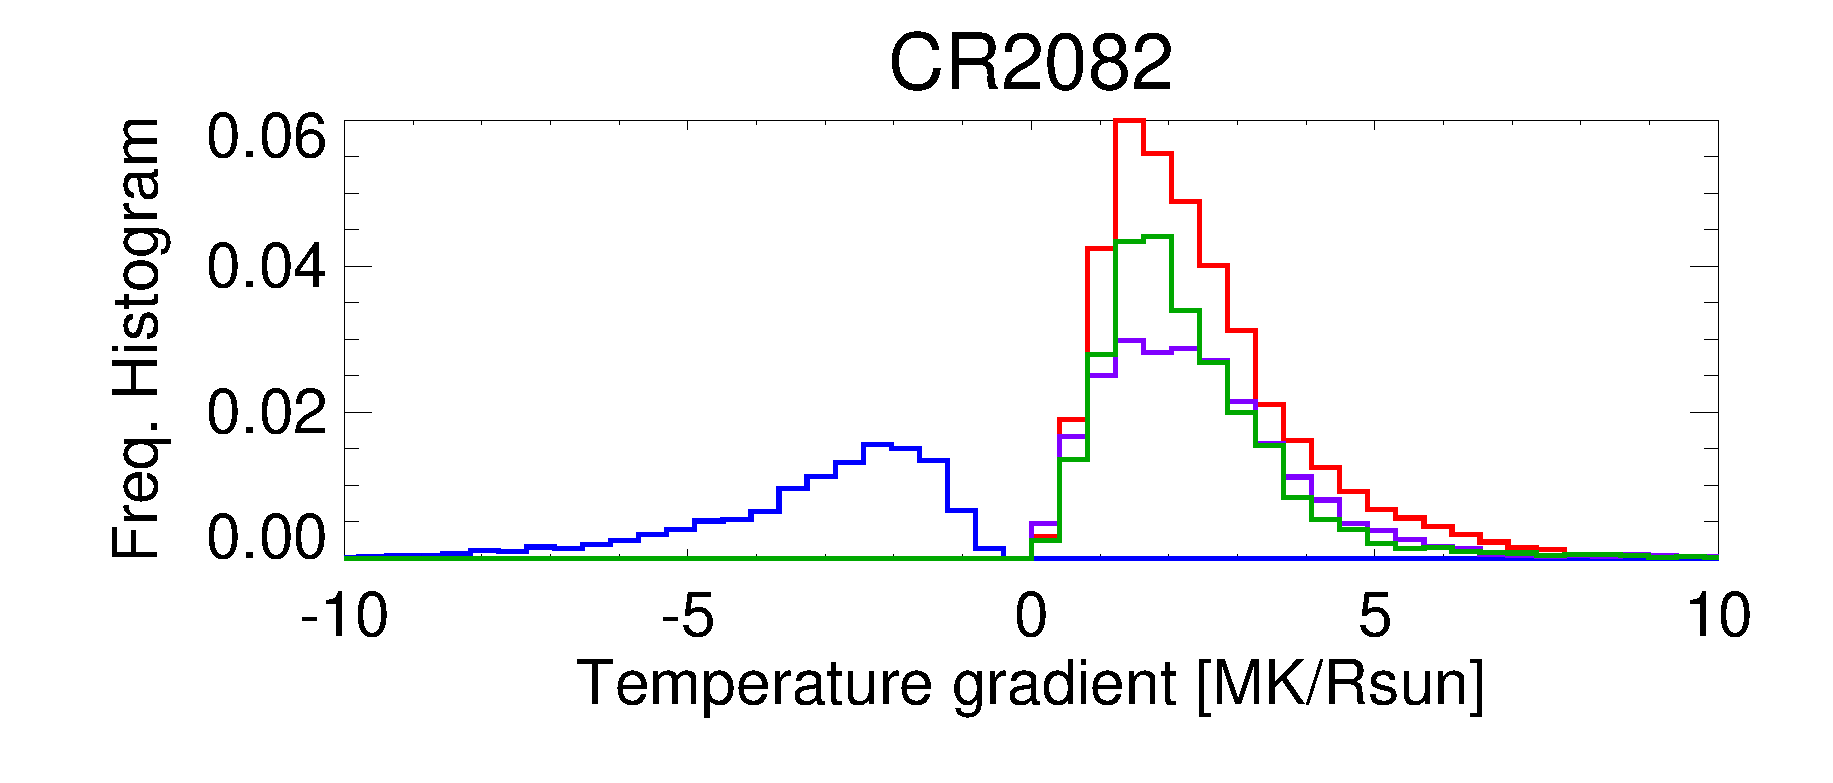
\includegraphics[width=0.495\textwidth,clip=]{figs/histo_cr2082_fulltriple_gradt.eps}
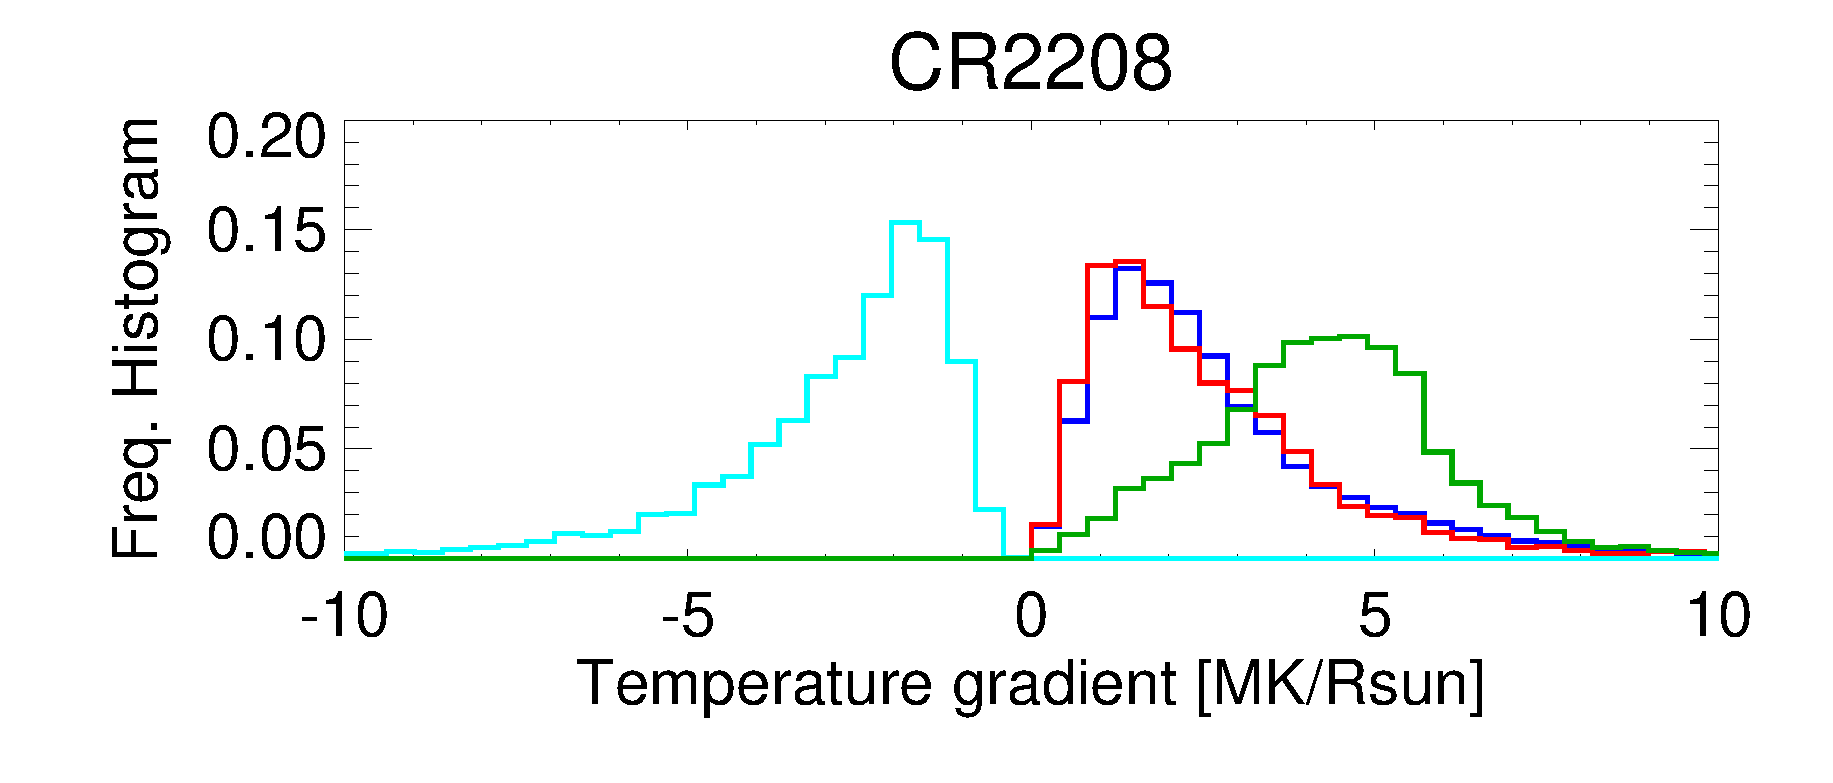
\includegraphics[width=0.495\textwidth,clip=]{figs/histo_cr2208_fulltriple_gradt.eps}
\caption{Frequency histograms of the temperature radial gradient for the different types of legs shown in Figure \ref{rpoint_demt} (same colour code) for CR-2082 (left panel) and CR-2208 (right panel).}
\label{gradt_demt}
\end{center}
\end{figure} 


As an example of the traced magnitudes, Figure \ref{histos_fulldemt} shows the statistical results of both rotations for all field lines types. From top to bottom type 0 to type 4. From left to right the panels show the statistical distribution of $\NCB$, $\lN$, $\aTm$, in each panel the median $m$ is indicated.


\begin{figure}[h!]
\begin{center}
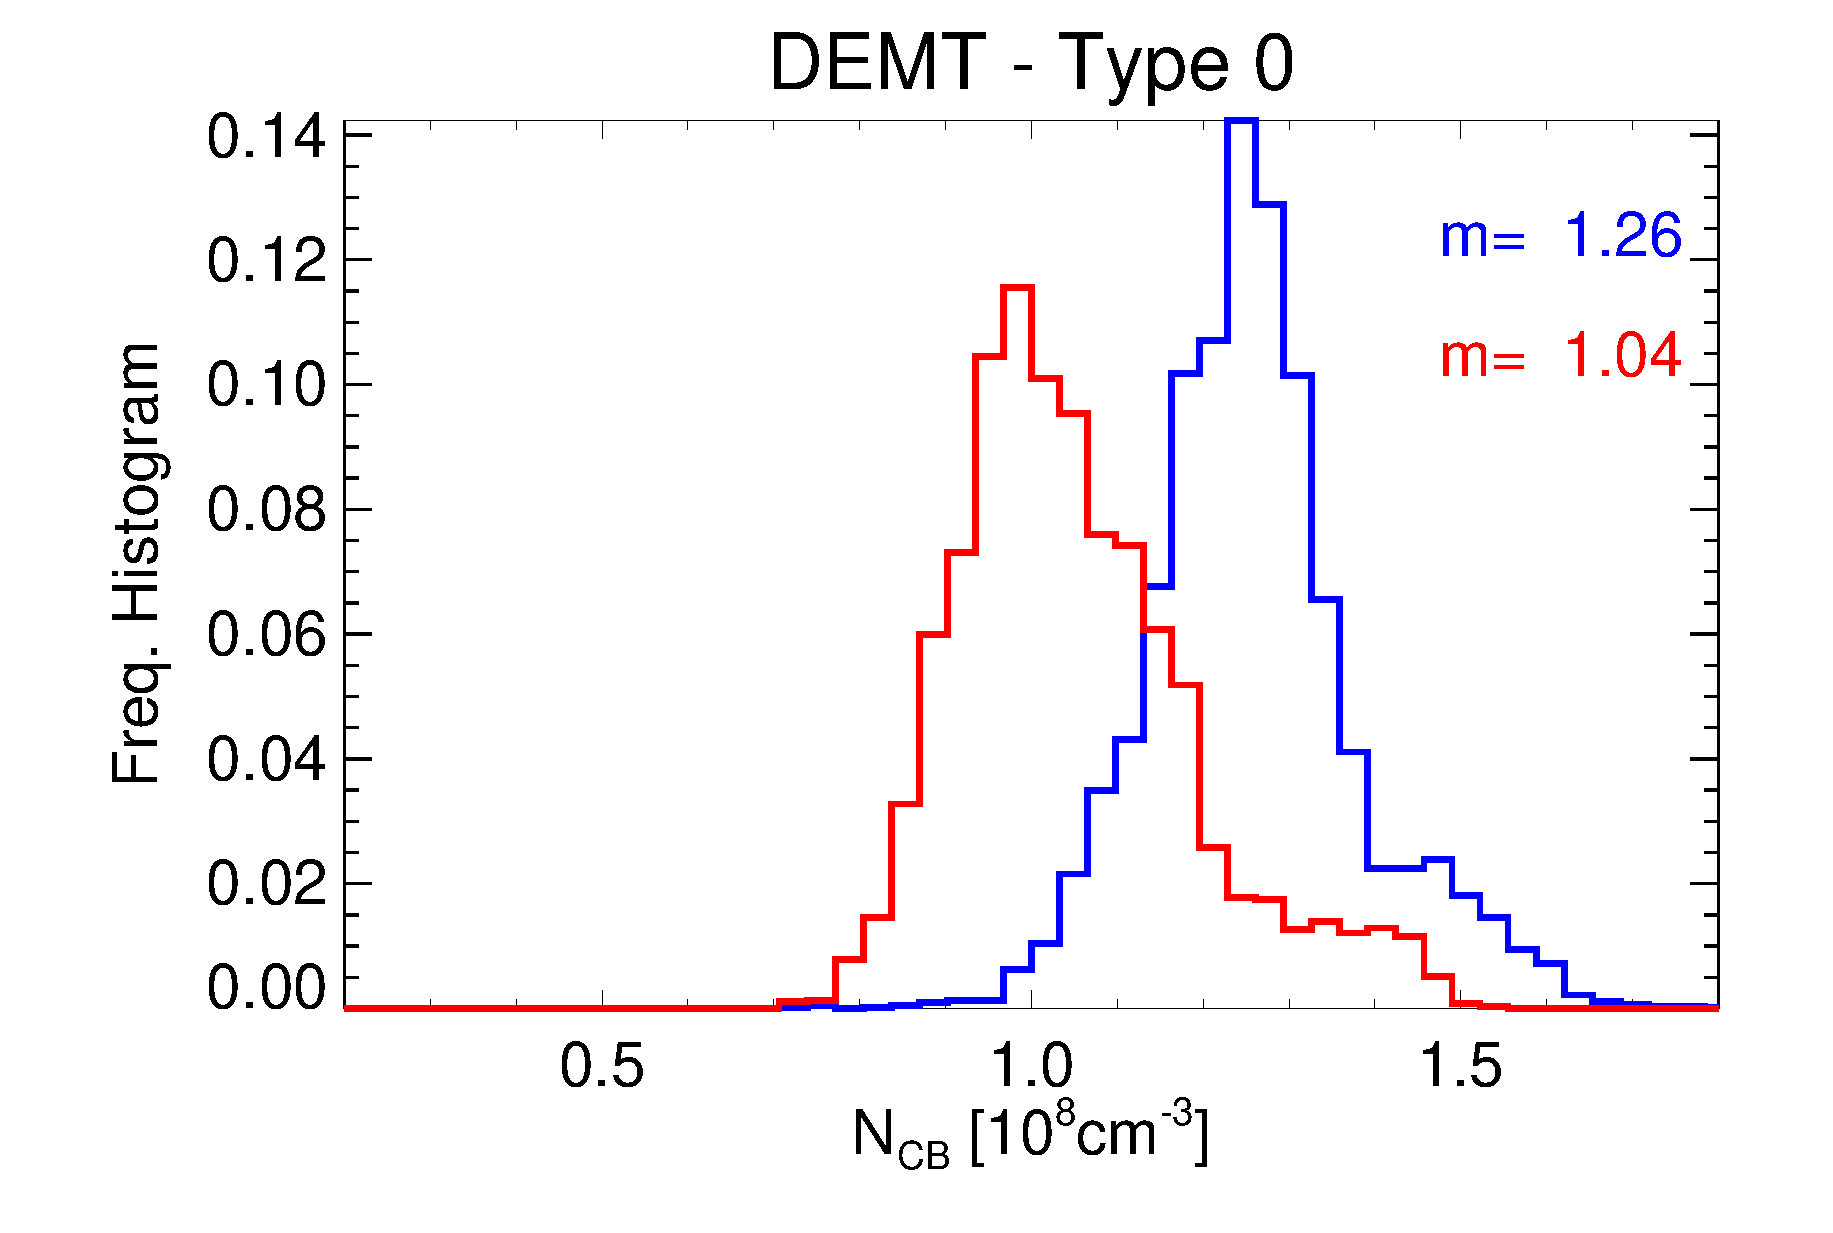
\includegraphics[width=0.31\textwidth,clip=]{figs/histo_2082_2208_fulldemt_streamer_down_ne_1055.eps}
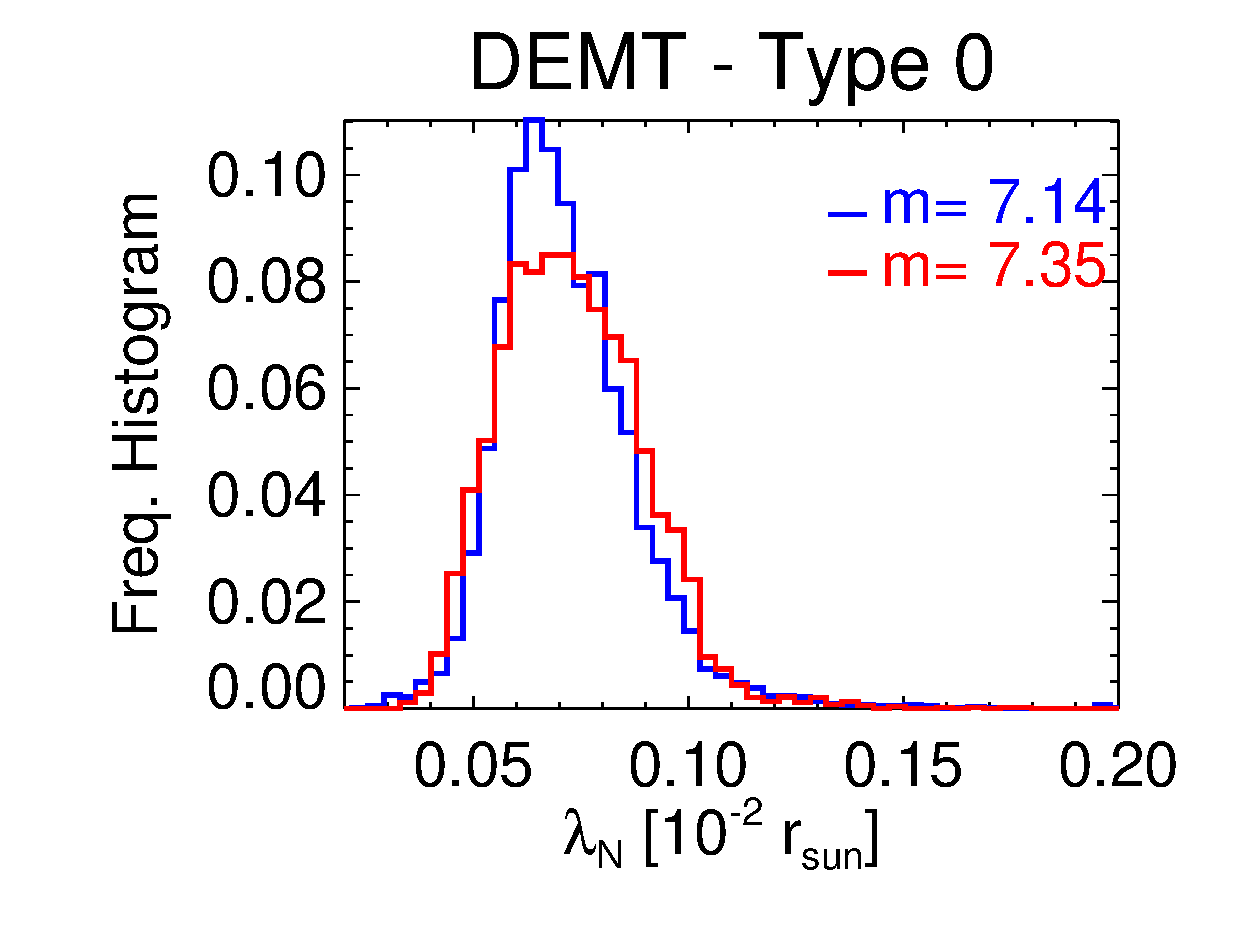
\includegraphics[width=0.31\textwidth,clip=]{figs/histo_2082_2208_fulldemt_streamer_down_lambda_n.eps}
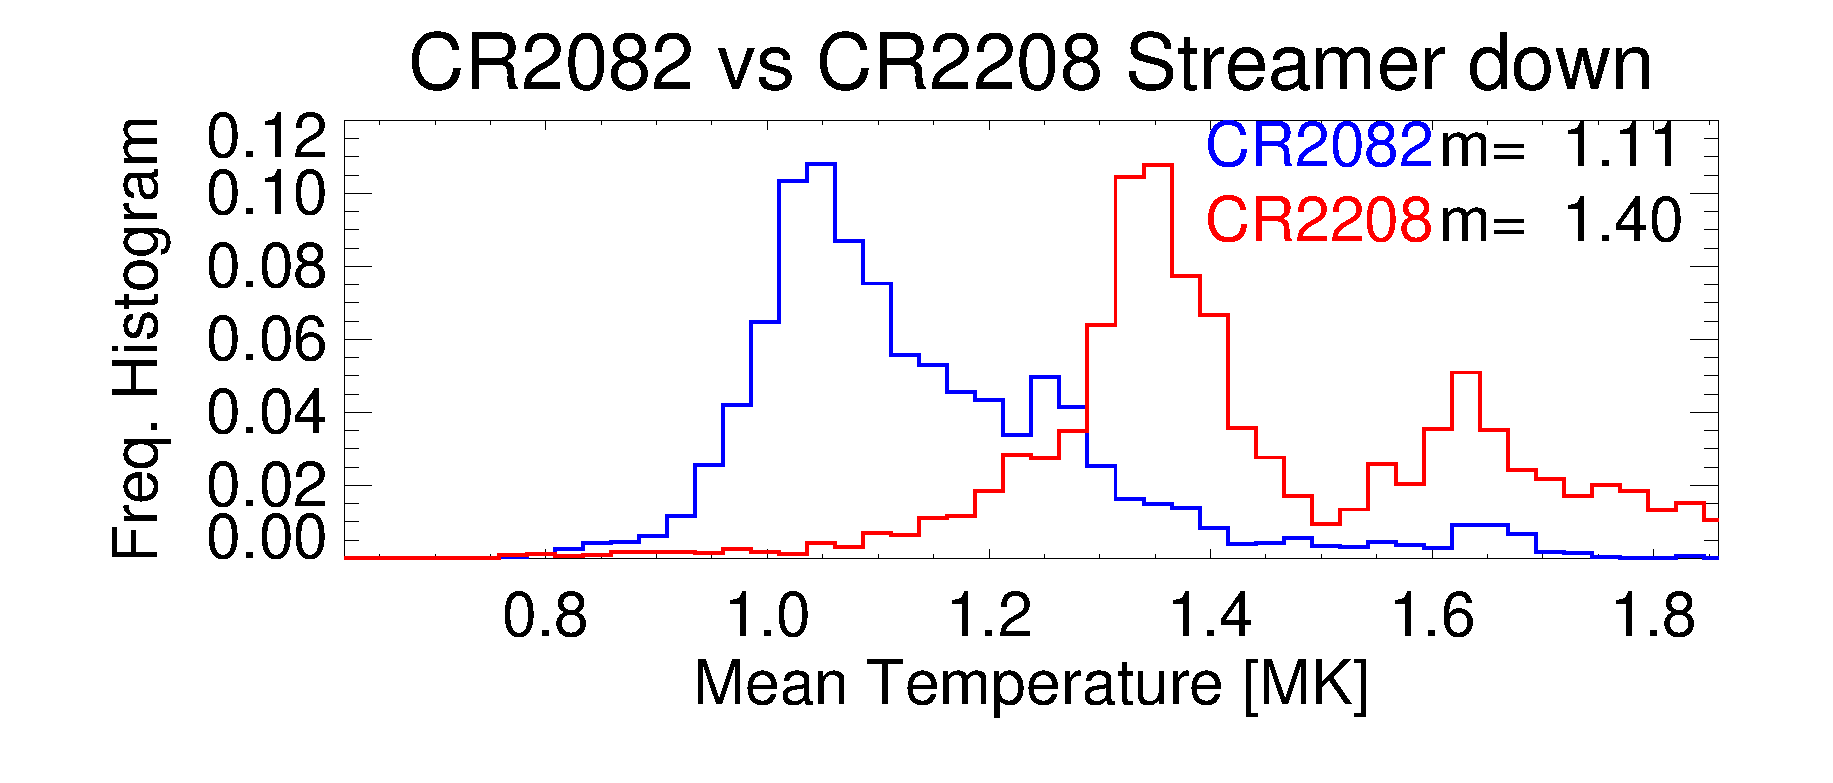
\includegraphics[width=0.31\textwidth,clip=]{figs/histo_2082_2208_fulldemt_streamer_down_Tm.eps}
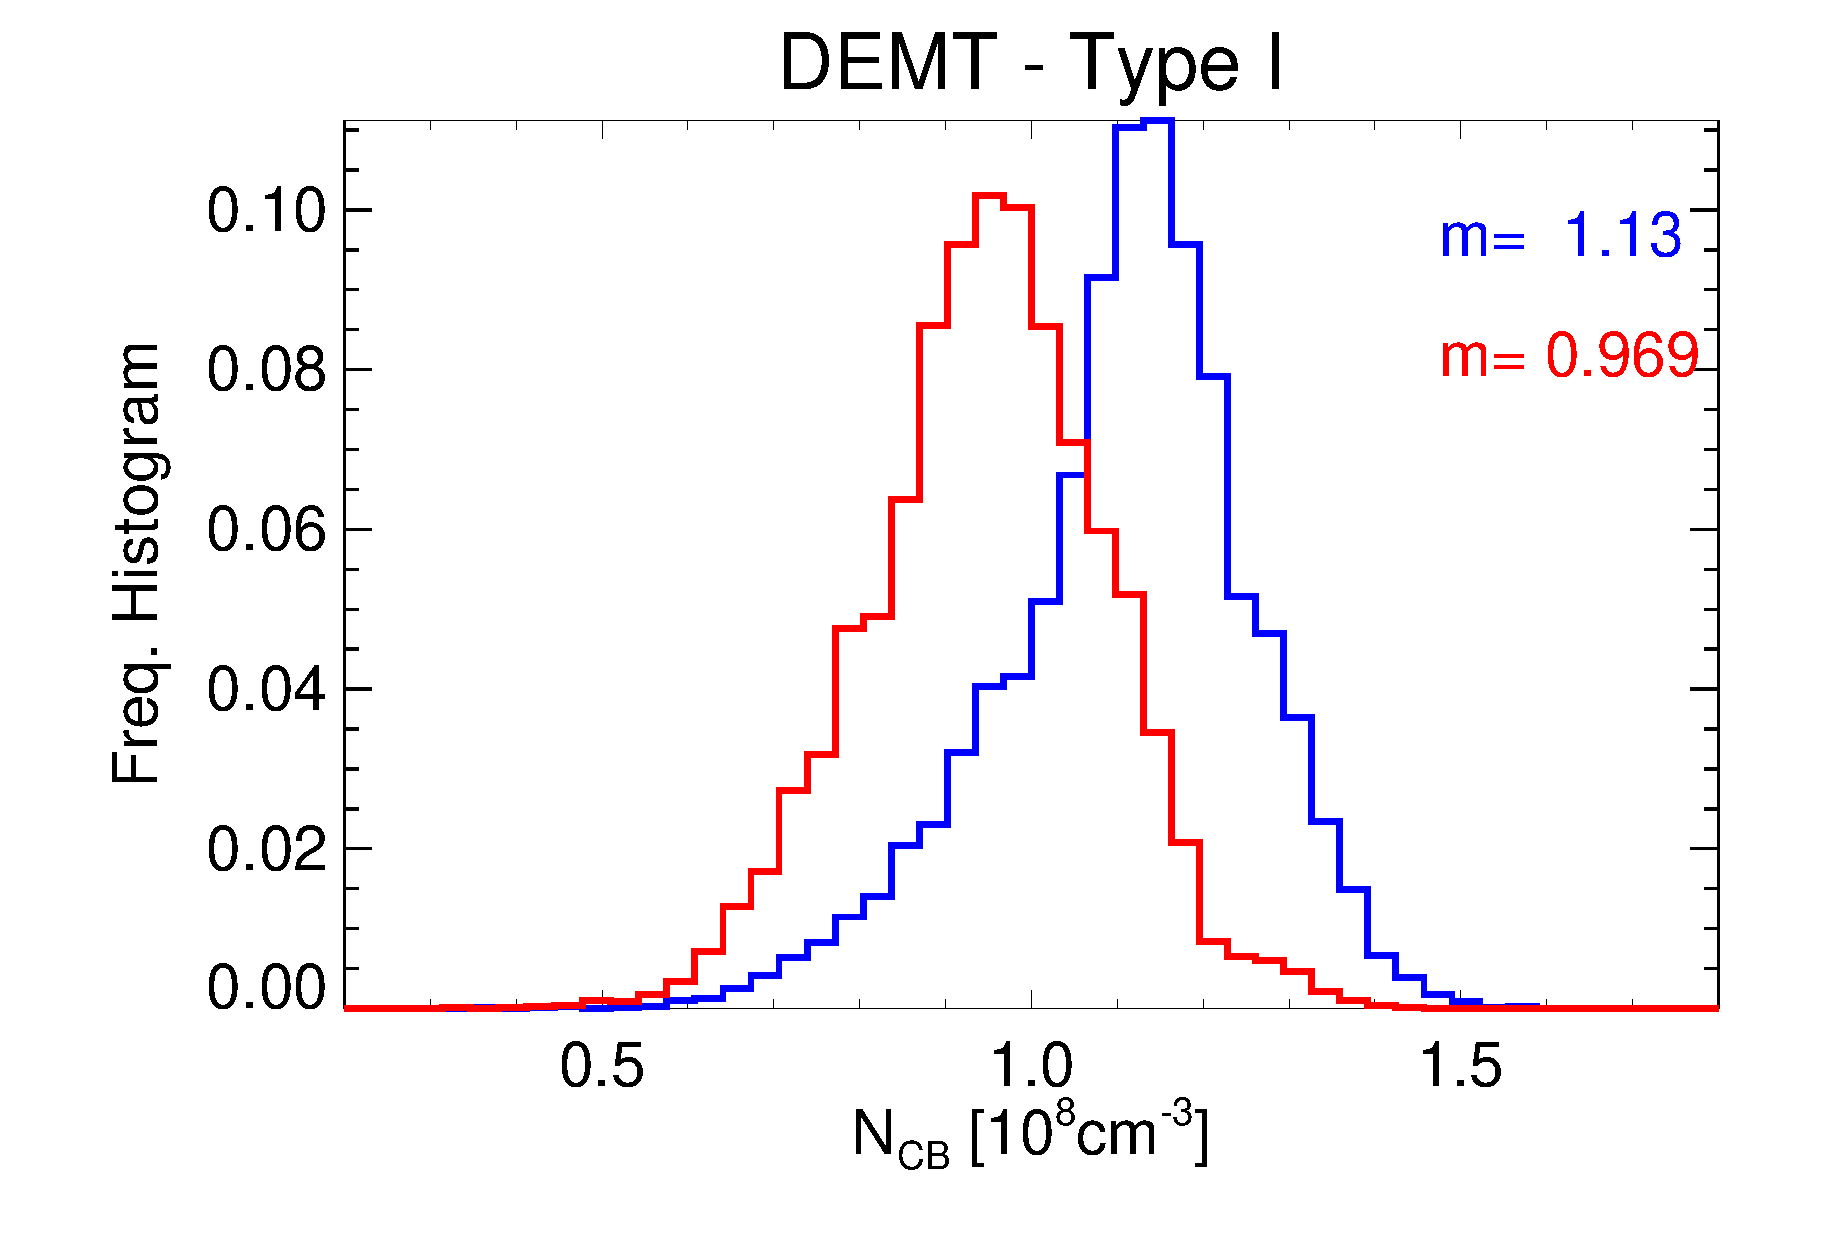
\includegraphics[width=0.31\textwidth,clip=]{figs/histo_2082_2208_fulldemt_streamer_up_ne_1055.eps}
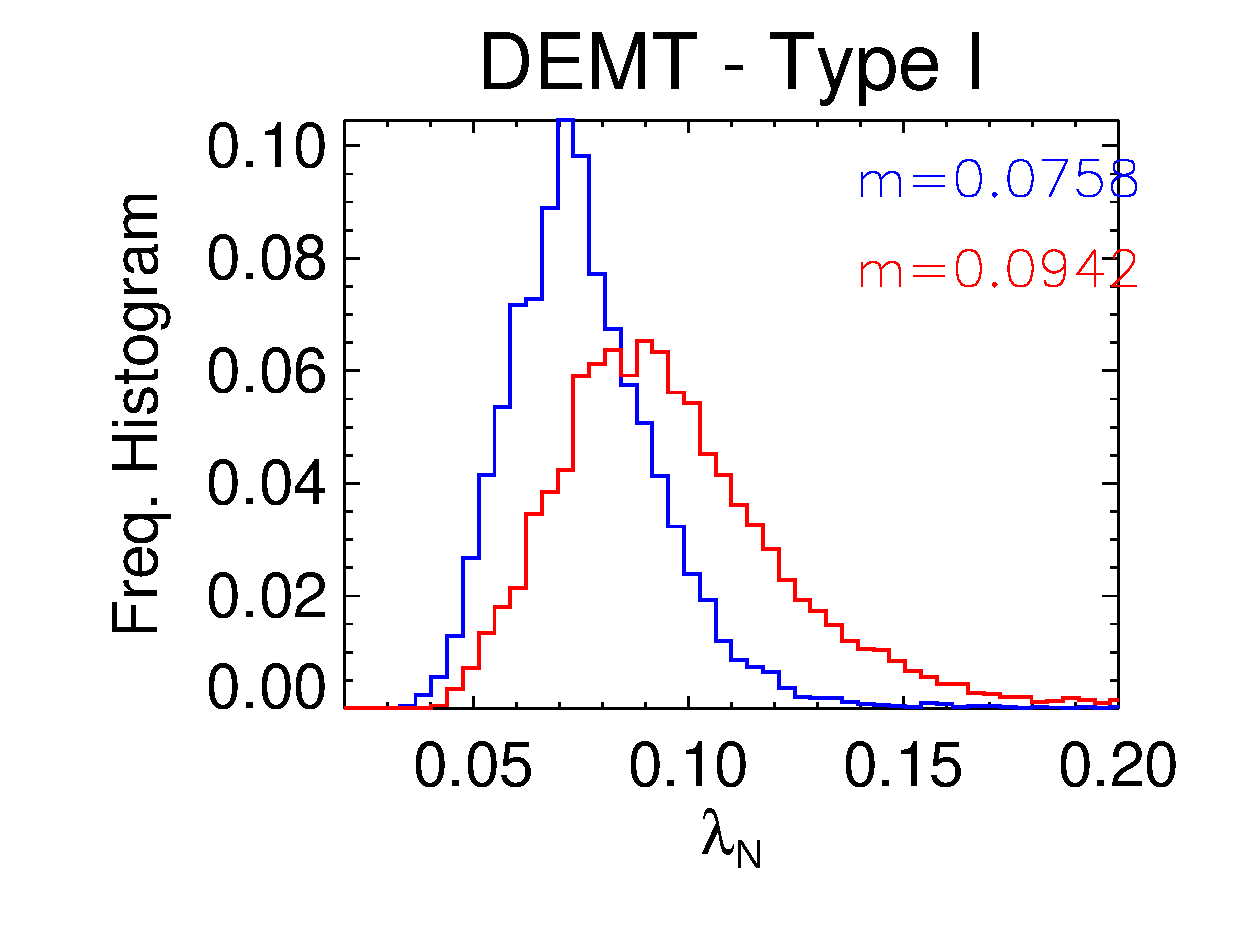
\includegraphics[width=0.31\textwidth,clip=]{figs/histo_2082_2208_fulldemt_streamer_up_lambda_n.eps}
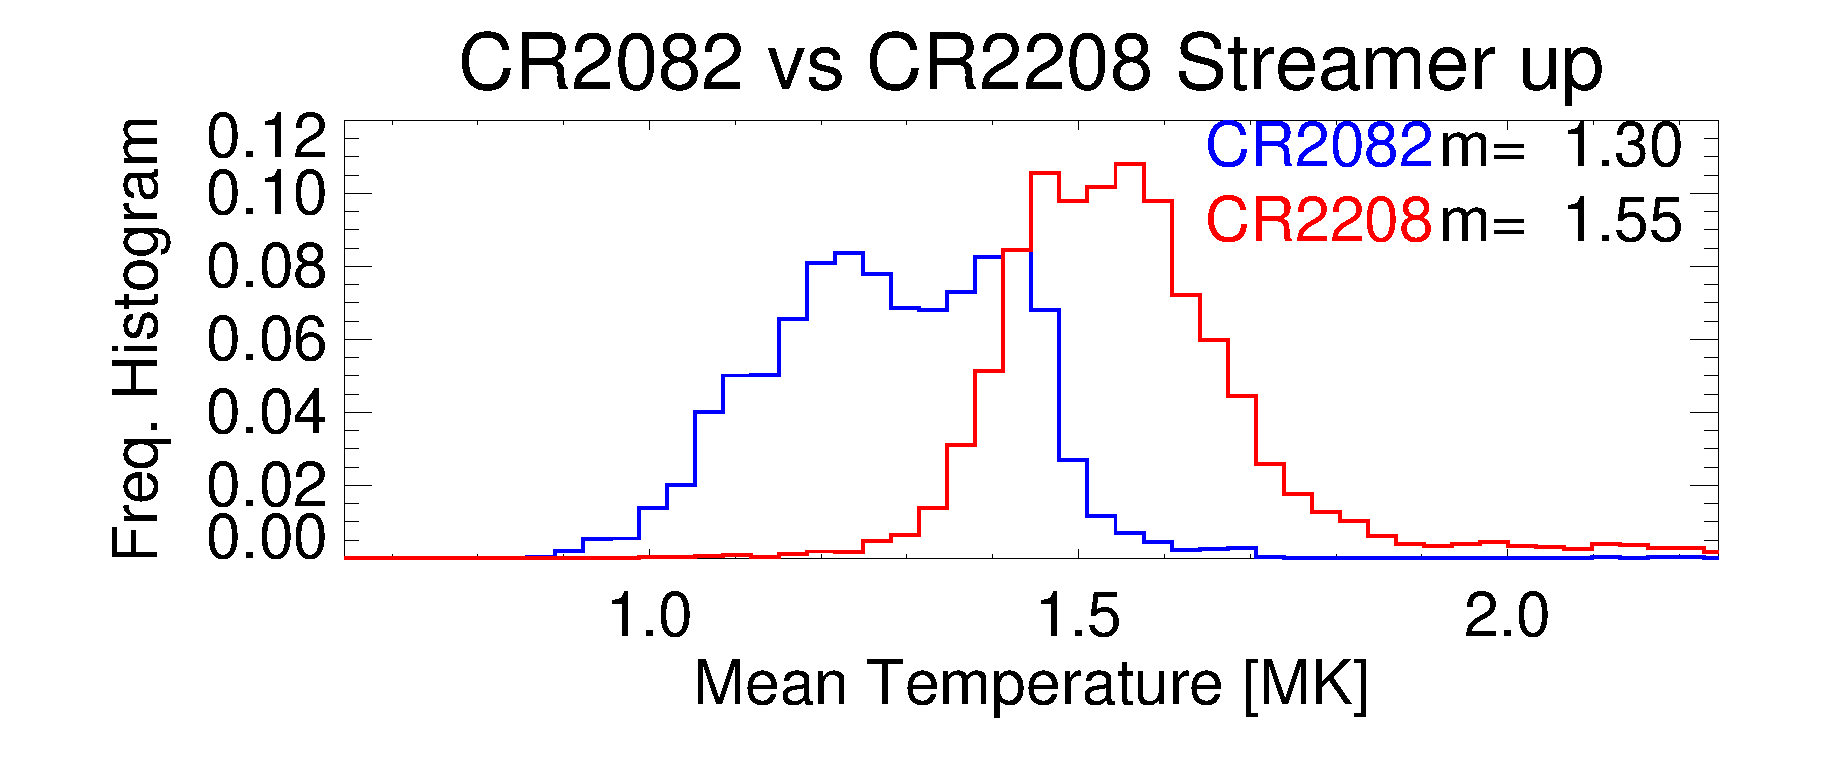
\includegraphics[width=0.31\textwidth,clip=]{figs/histo_2082_2208_fulldemt_streamer_up_Tm.eps}
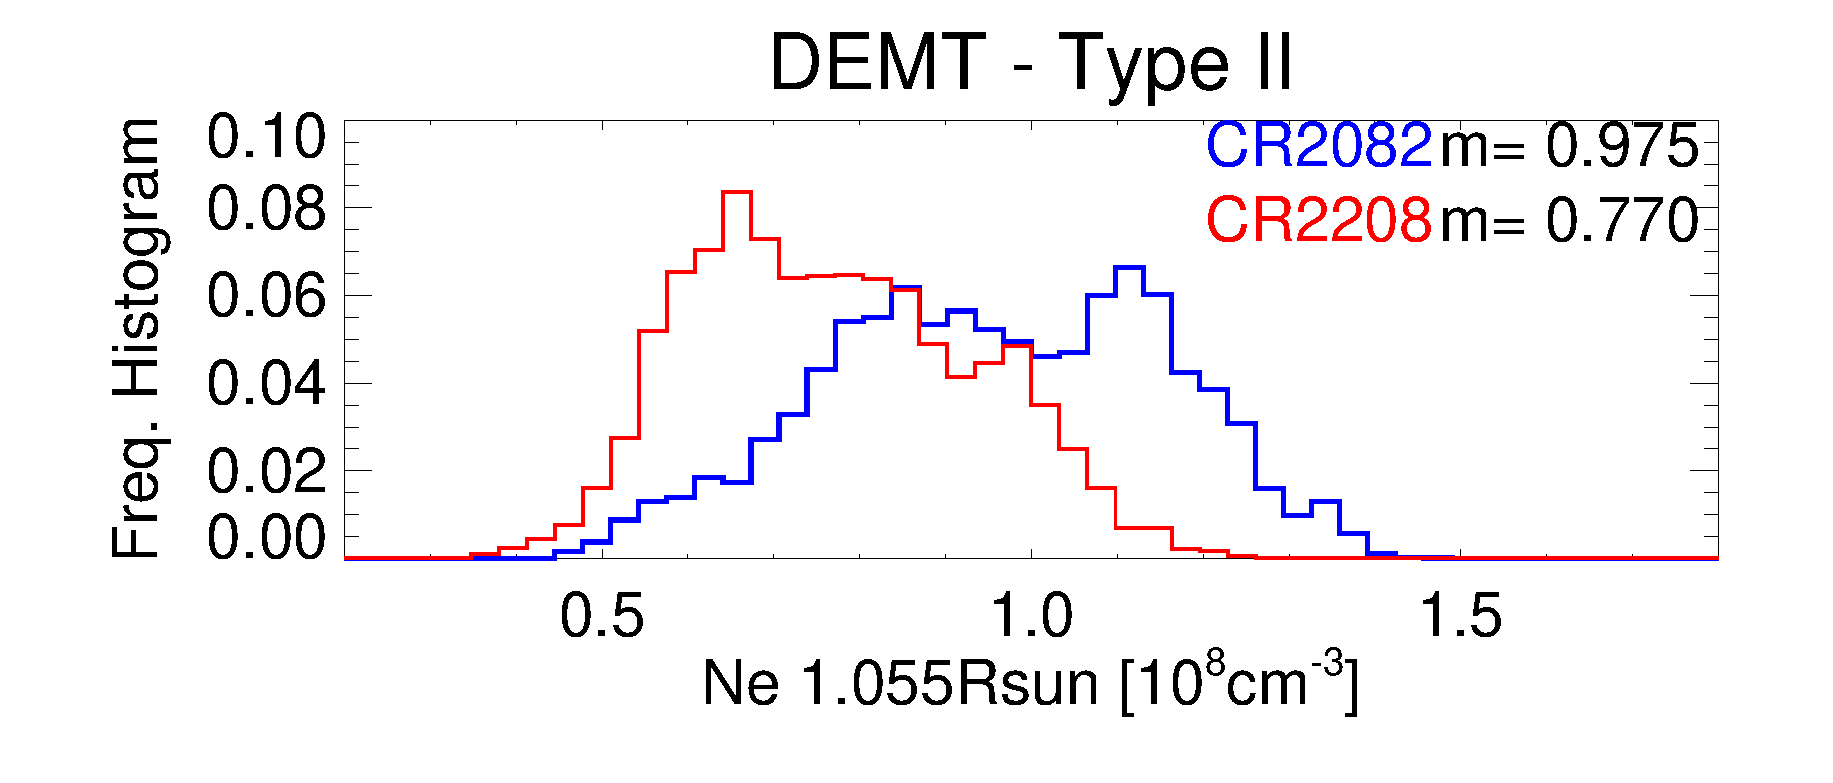
\includegraphics[width=0.31\textwidth,clip=]{figs/histo_2082_2208_fulldemt_bound_up_ne_1055.eps}
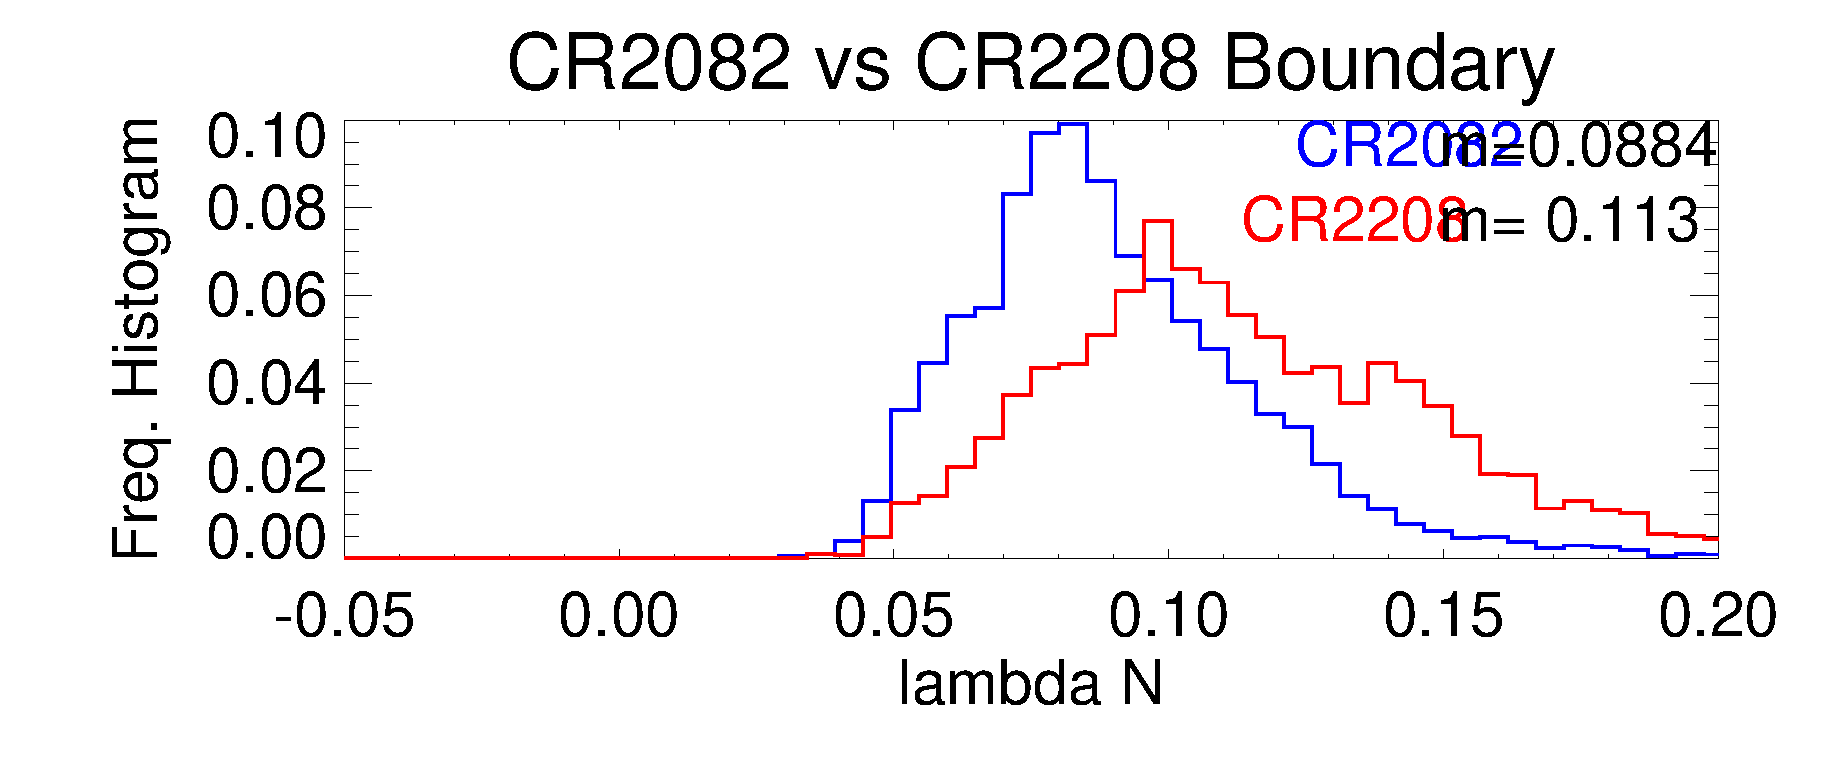
\includegraphics[width=0.31\textwidth,clip=]{figs/histo_2082_2208_fulldemt_bound_up_lambda_n.eps}
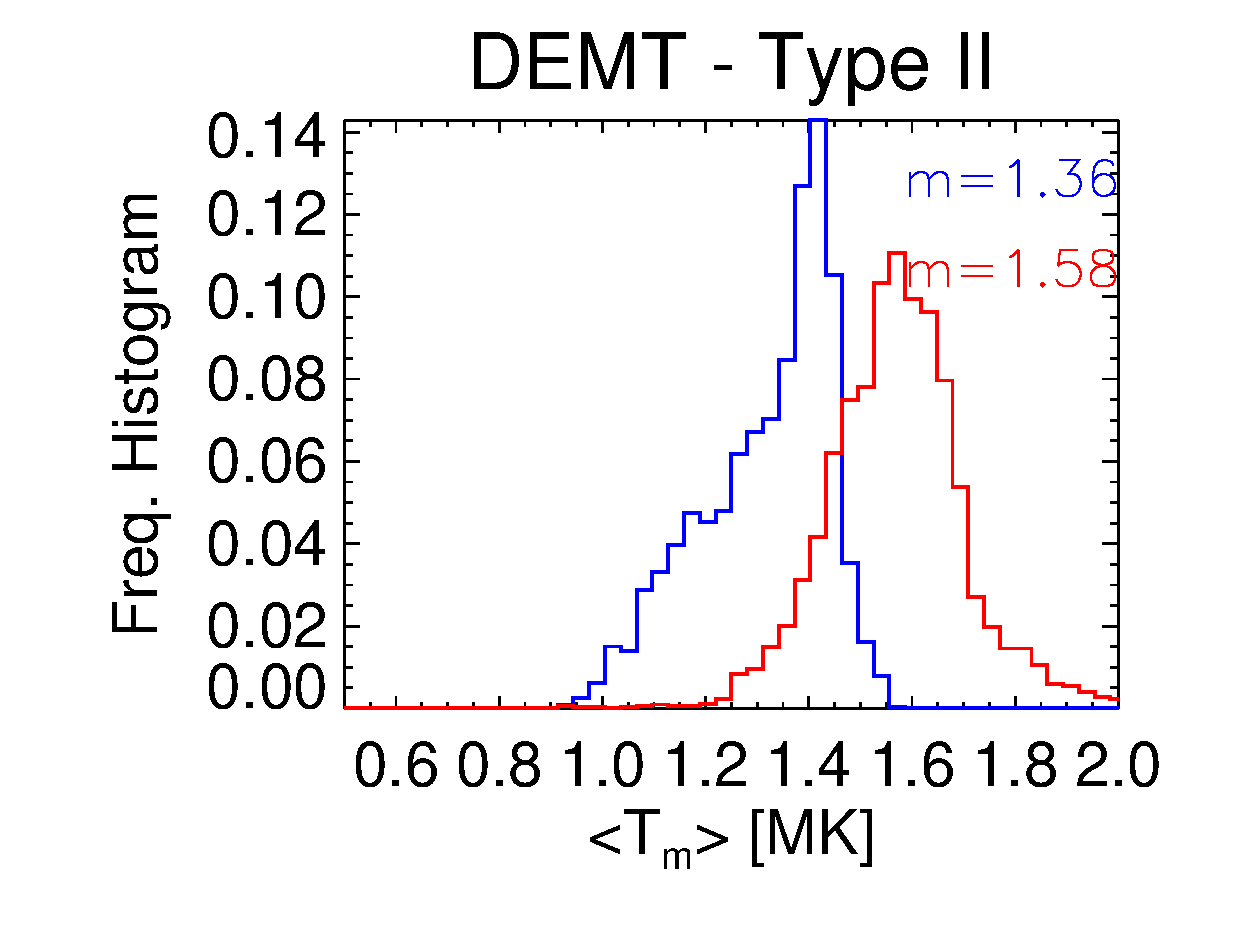
\includegraphics[width=0.31\textwidth,clip=]{figs/histo_2082_2208_fulldemt_bound_up_Tm.eps}
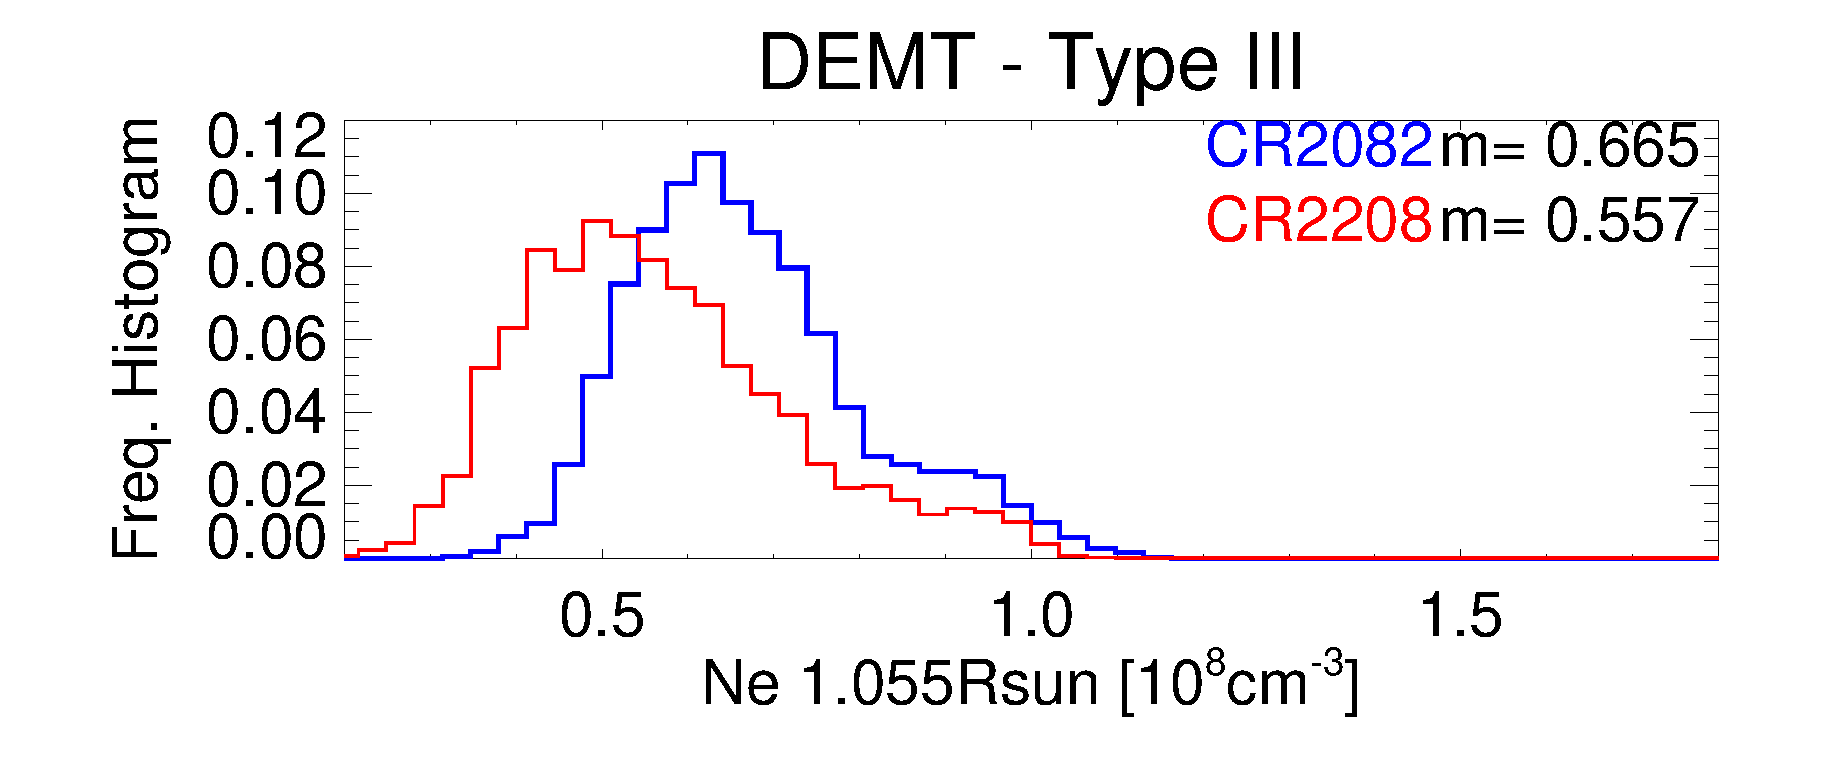
\includegraphics[width=0.31\textwidth,clip=]{figs/histo_2082_2208_fulldemt_CH_up_ne_1055.eps}
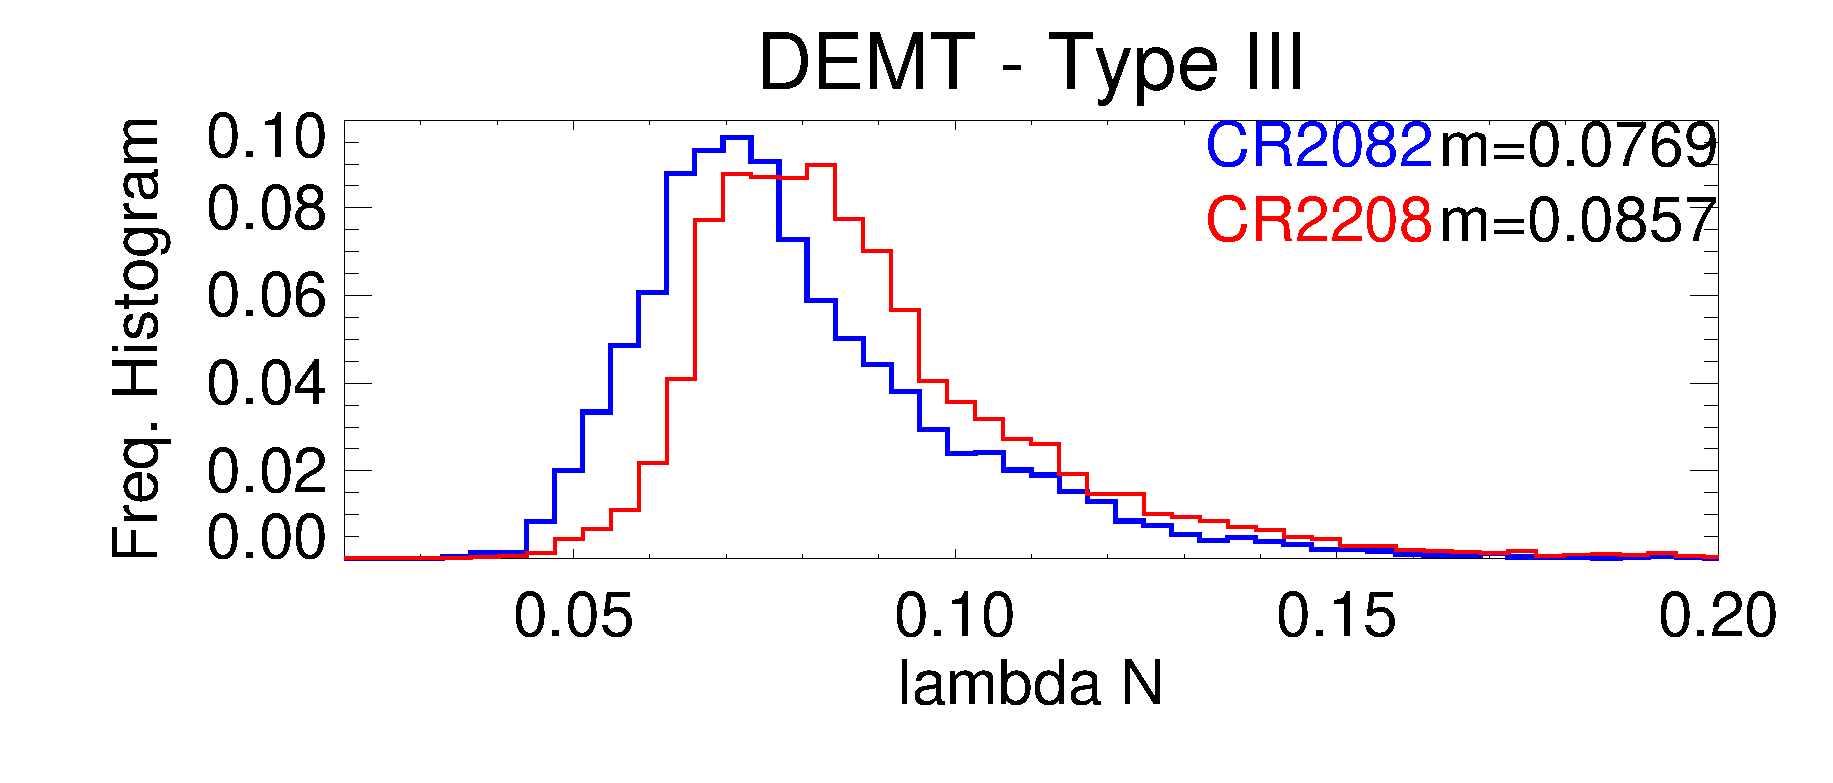
\includegraphics[width=0.31\textwidth,clip=]{figs/histo_2082_2208_fulldemt_CH_up_lambda_n.eps}
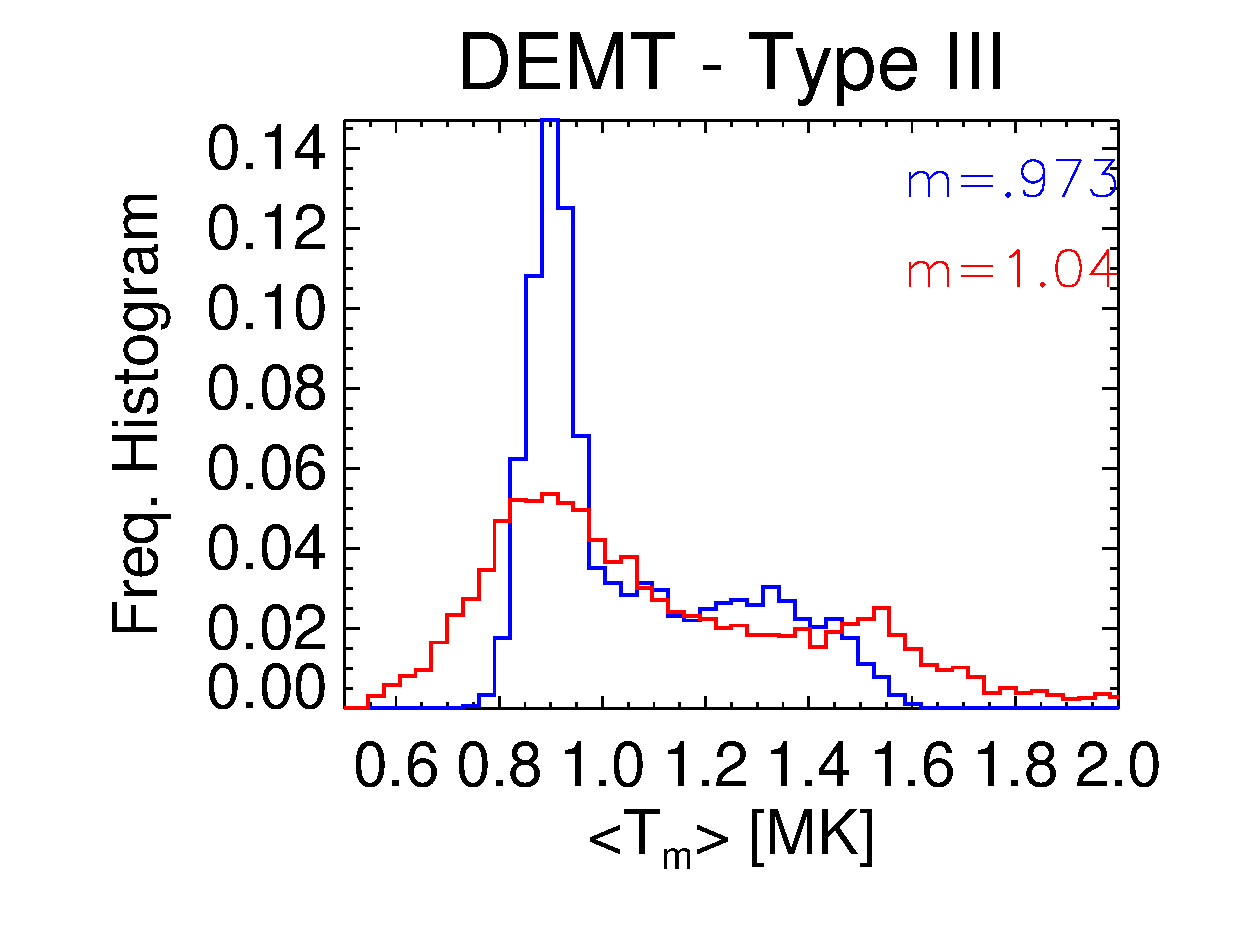
\includegraphics[width=0.31\textwidth,clip=]{figs/histo_2082_2208_fulldemt_CH_up_Tm.eps}
\caption{Comparative statistical distributions of DEMT reults. From left to right: the coronal base electron density $\Ne(r=1.055\,\mrsun)$, the electron density scale height $\lN$ and the average electron mean temperature $\aTm$, along all types of legs defined in Section \ref{trace}. Results of CR2082 are shown in blue while those of CR-2208 in red. In each panel the median $m$ is indicated.}
\label{histos_fulldemt}
\end{center}
\end{figure} 

For all type of lines, Table \ref{tabla_demt} summarize the quantitative comparative analysis between the results of the two target rotations sampling both minima. For CR-2082 quantities are expressed as absoulte values, qhile for CR-2208 they are informed relative to the corresponding results for CR-2082. The following major results concerning the structure of each rotation individually and their comparison can be drawn.

\begin{table}
\begin{tabular}{l r@{.}l@{\hskip 0.05in} r@{\hskip 0.01in} r@{.}l  r@{.}l@{\hskip 0.05in} r@{\hskip 0.01in} r@{.}l r@{.}l@{\hskip 0.05in} r@{\hskip 0.01in} r@{.}l }
% r@{.}l@{\hskip 0.05in} r@{\hskip 0.01in} r@{.}l@{\hskip 0.01in} l}
\hline
Type    & \multicolumn{5}{c}{$\med(\NCB)$}             & \multicolumn{5}{c}{$\med(\lN)$} & \multicolumn{5}{c}{$\med(\avgTe)$} \\
       & \multicolumn{5}{c}{$[10^8\,{\rm cm}^{-3}]$}  & \multicolumn{5}{c}{$[{\rm 10}^{-2}\,\mrsun]$} & \multicolumn{5}{c}{$[\MK]$} \\
\hline
0  & 0&93 &(\Mi&12&9\%)  &   7&4 &(\Pl&~3&9\%) &   1&11 &(\Pl&20&7\%) \\
1  & 0&84 &(\Mi&11&3\%)  &   8&3 &(\Pl&15&3\%) &   1&30 &(\Pl&16&1\%) \\
2  & 0&74 &(\Mi&16&1\%)  &   8&9 &(\Pl&19&1\%) &   1&33 &(\Pl&14&2\%) \\
3  & 0&48 &(\Mi&12&5\%)  &   7&7 &(\Pl&10&5\%) &   0&98 &(\Pl&~5&7\%) \\
\hline          
\end{tabular}
\caption{Median value (indicated as ``Md'') of the statistical distribution of $\NCB$, $\lN$, and $\aTm$ for each coronal type of lines defined in Section \ref{trace}. For CR-2082 values are expressed in absolute terms, while for CR-2208 they are informed as a percentual variation relative to the CR-2082 value.}
\label{tabla_demt}
\end{table}


In the equatorial streamer of both rotations, increasing latitudes show decreasing \temp{coronal base (1.055)} density, and increasing density scale height and electron temperature. In both rotations the CH regions are characterized sub-MK temperatures, and coronal base densities of order $\approx 1/2$ of the equatorial streamer. Histograms with sharp populations indicates that for both rotations the values of all physical quantities exhibit a strong symmetry between both hemispheres.

A comparison of the results between the two rotations within the closed field lines \temp{equatorial streamer belt} shows that CR-2208 is characterized by lower values of electron density and larger of temperature compared to CR-2082, as well as larger values of the density scale height.
\temp{Comentario sobre la estimacion de errores del paper pasado?}

In the coronal hole region, \temp{No se si se puede aclarar algo en particular, quizas decir que ahora que tomamos una gran region abierta (en comparacion con el paper pasado) la seleccion toma lineas en la transicion de viento lento y rapido y eso genera que el histograma de Tm sea tan disperso}

%To establish if the differences in the results between the two rotations are significant, Section \ref{uncertainties} estimates the error bars due the dominating systematic uncertainties.

%{Also, within the streamer belt the magnetic field strength is similar in both rotations in the northern hemisphere, while in the southern hemisphere CR-1915 exhibits $10-80\%$ larger values compared to CR-2081, with increasing difference for larger latitudes. In the coronal holes, the magnetic field strength of CR-1915 is much larger than for CR-2081, exhibiting values up to 50\% larger in the northern hemisphere and more than twice larger in the southern hemisphere.}

\temp{Aca vienen quizas 1 o 2 parrafos introduciendo y explicando los phi, los resultados de la Figura \ref{energia_demt} y un parrafo comentando esos resultados. Este parrafo va escrito por Ceci.}


\begin{figure}[h!]
\begin{center}
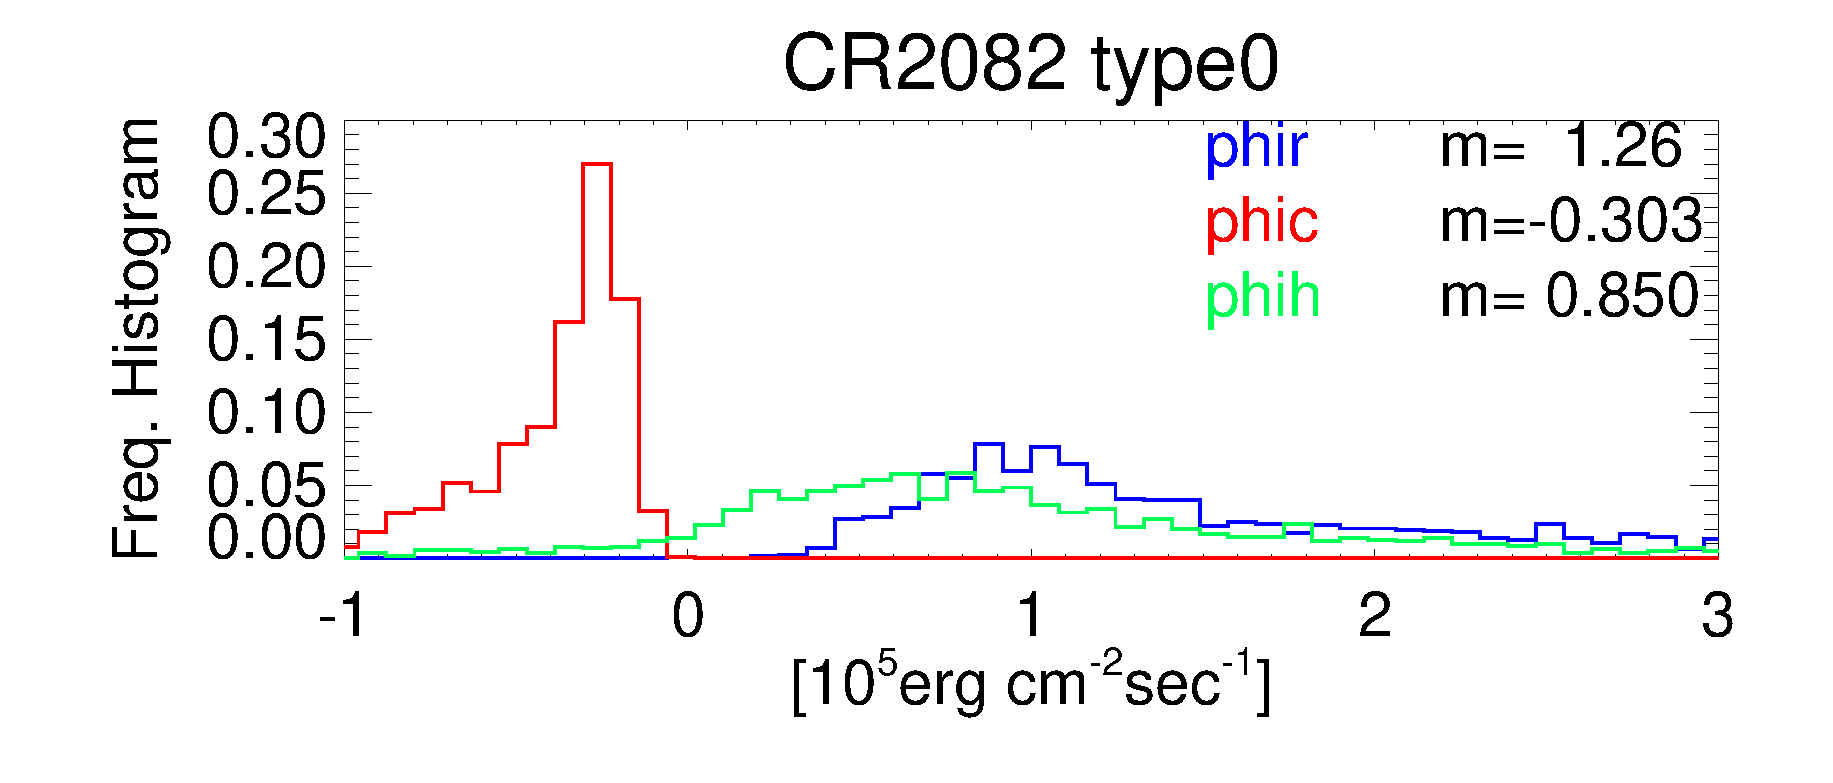
\includegraphics[width=0.495\textwidth,clip=]{figs/histocr2082_ccdownenergia.eps}
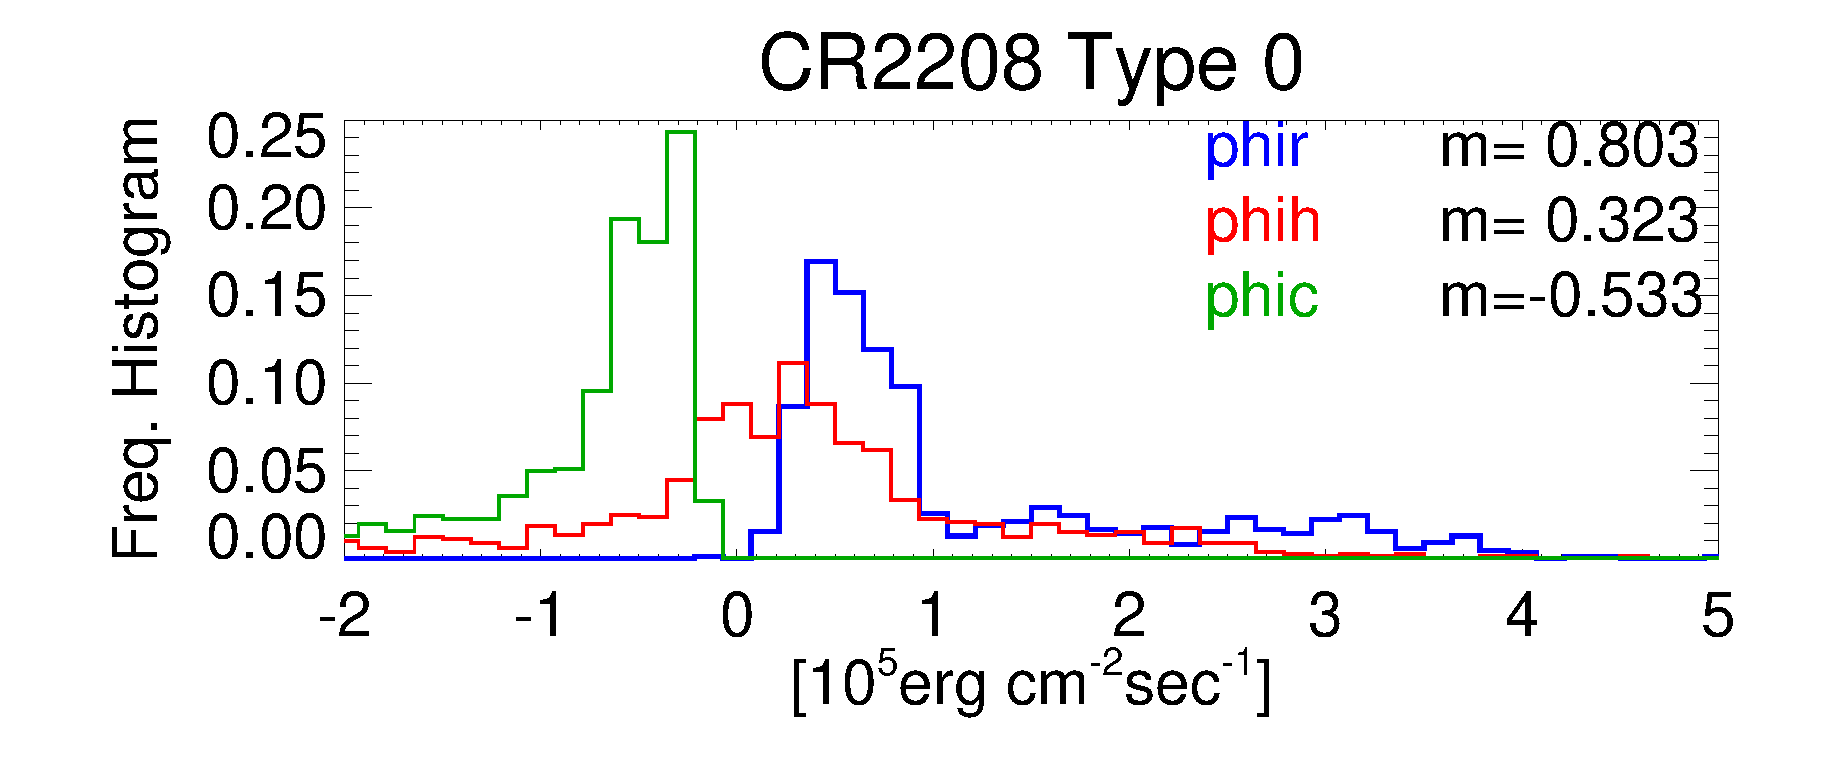
\includegraphics[width=0.495\textwidth,clip=]{figs/histocr2208_ccdownenergia.eps}
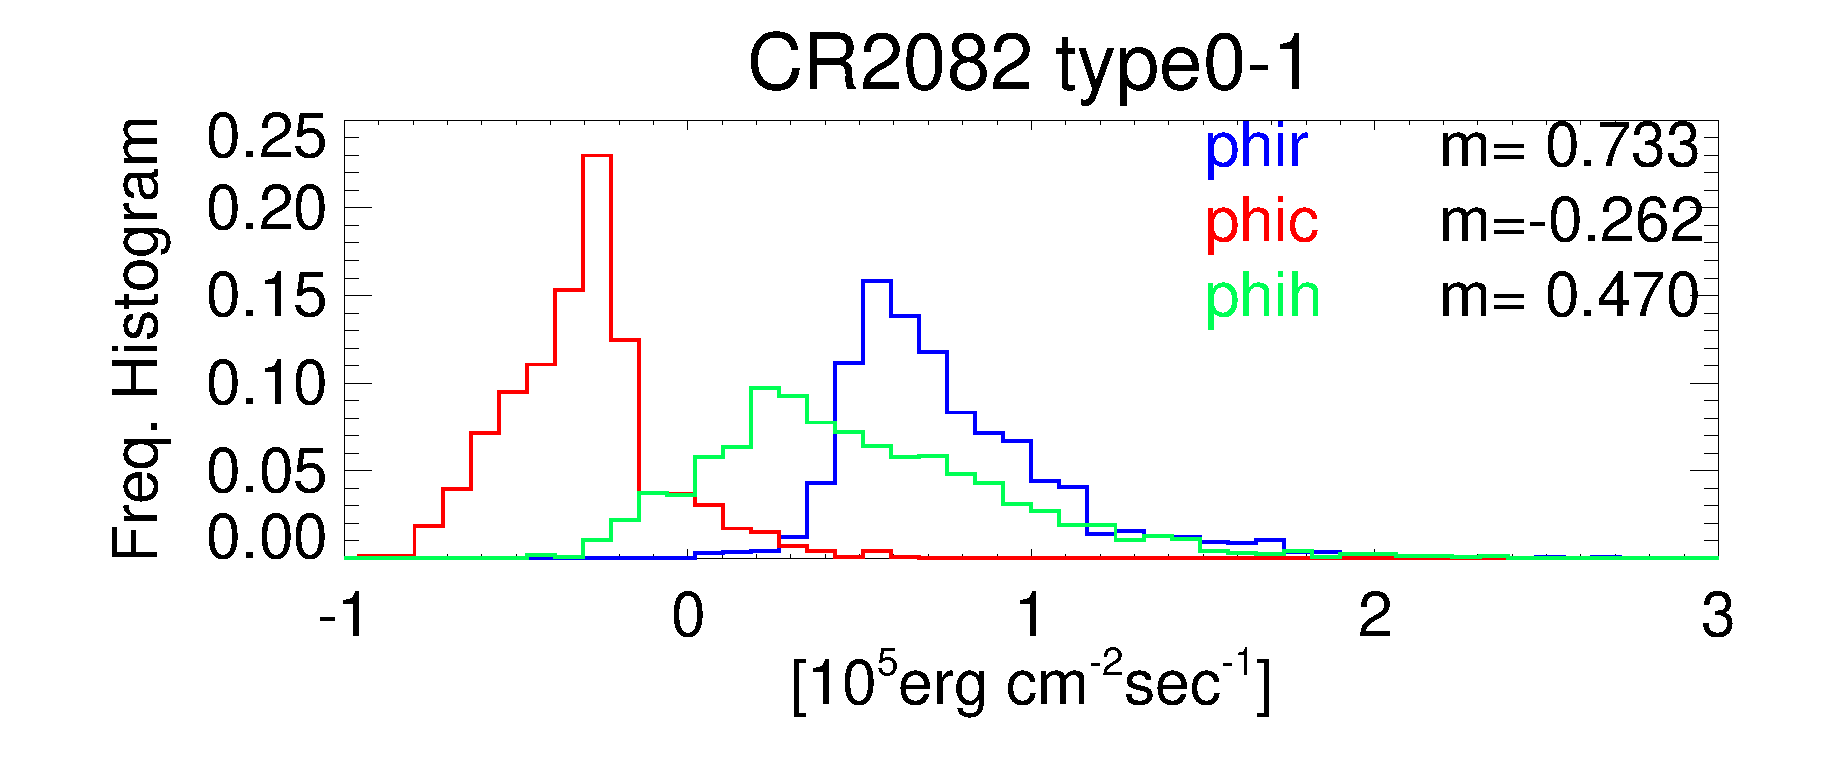
\includegraphics[width=0.495\textwidth,clip=]{figs/histocr2082_ccenergia.eps}
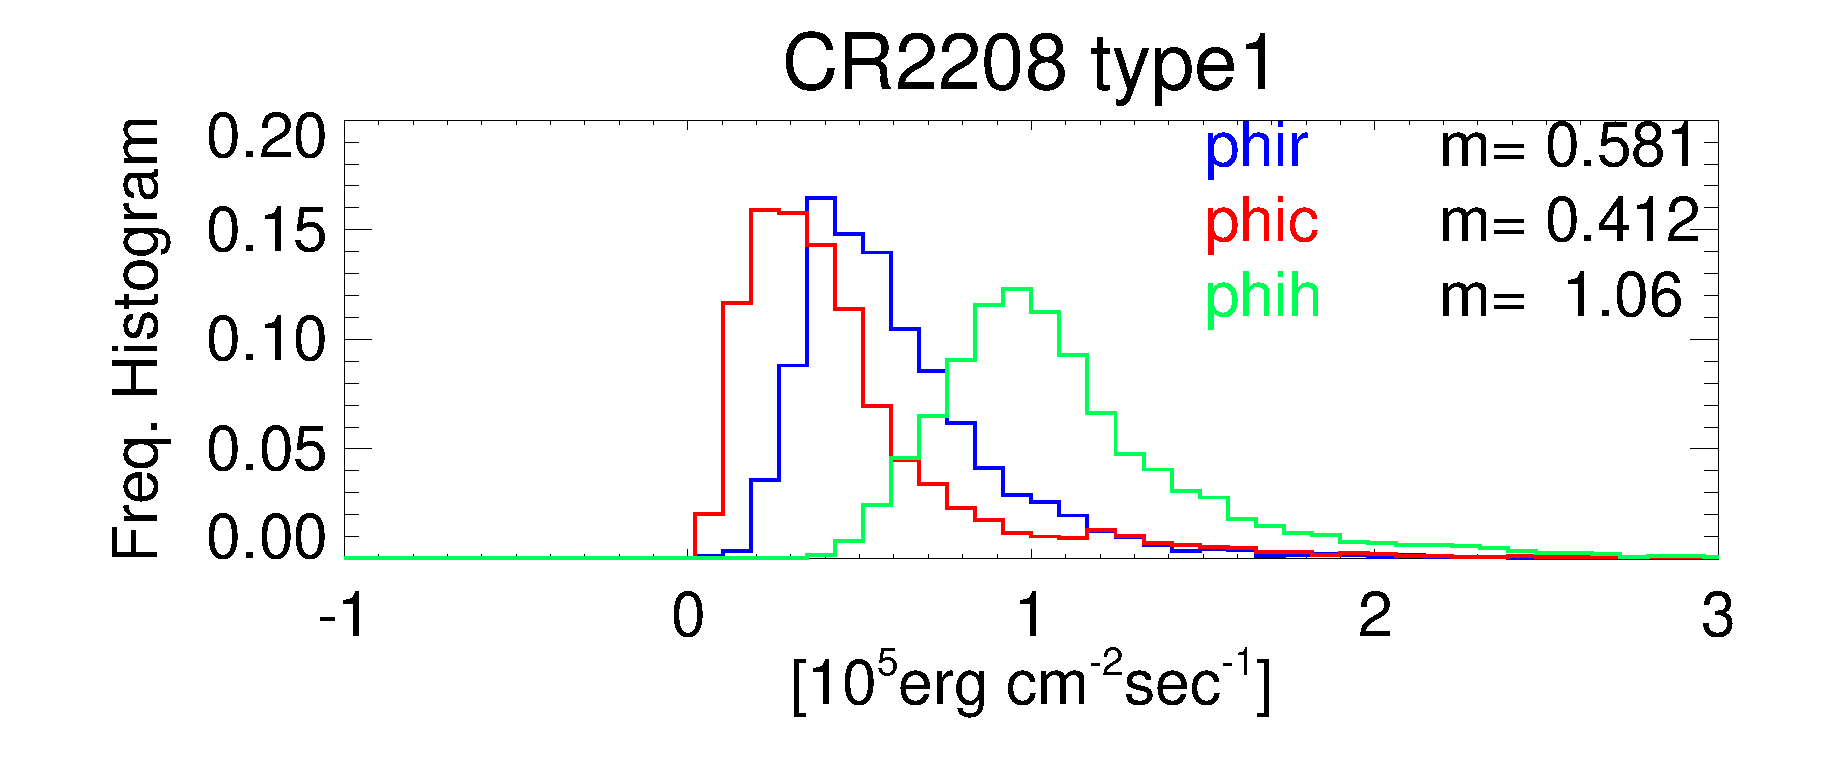
\includegraphics[width=0.495\textwidth,clip=]{figs/histocr2208_ccenergia.eps}
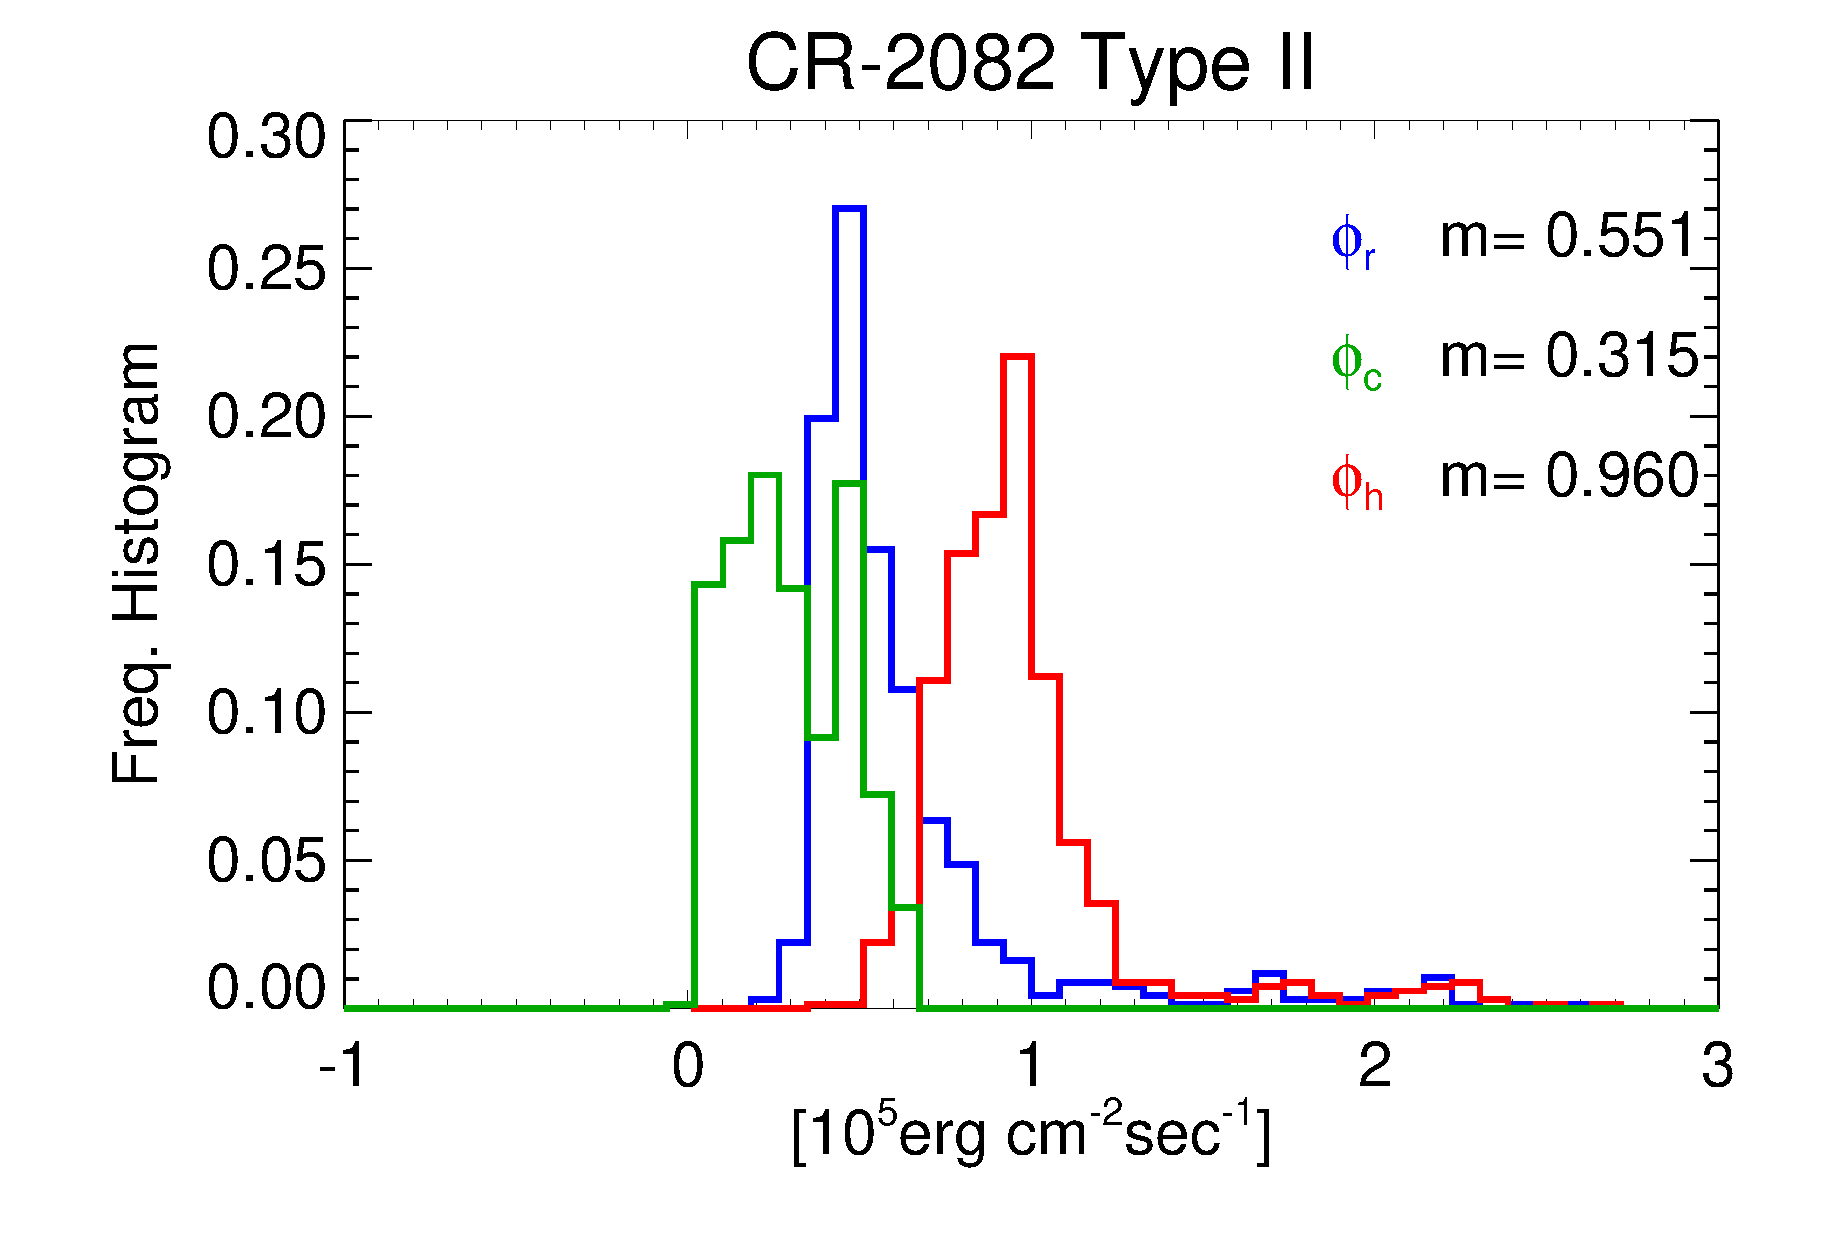
\includegraphics[width=0.495\textwidth,clip=]{figs/histocr2082_cgenergia.eps}
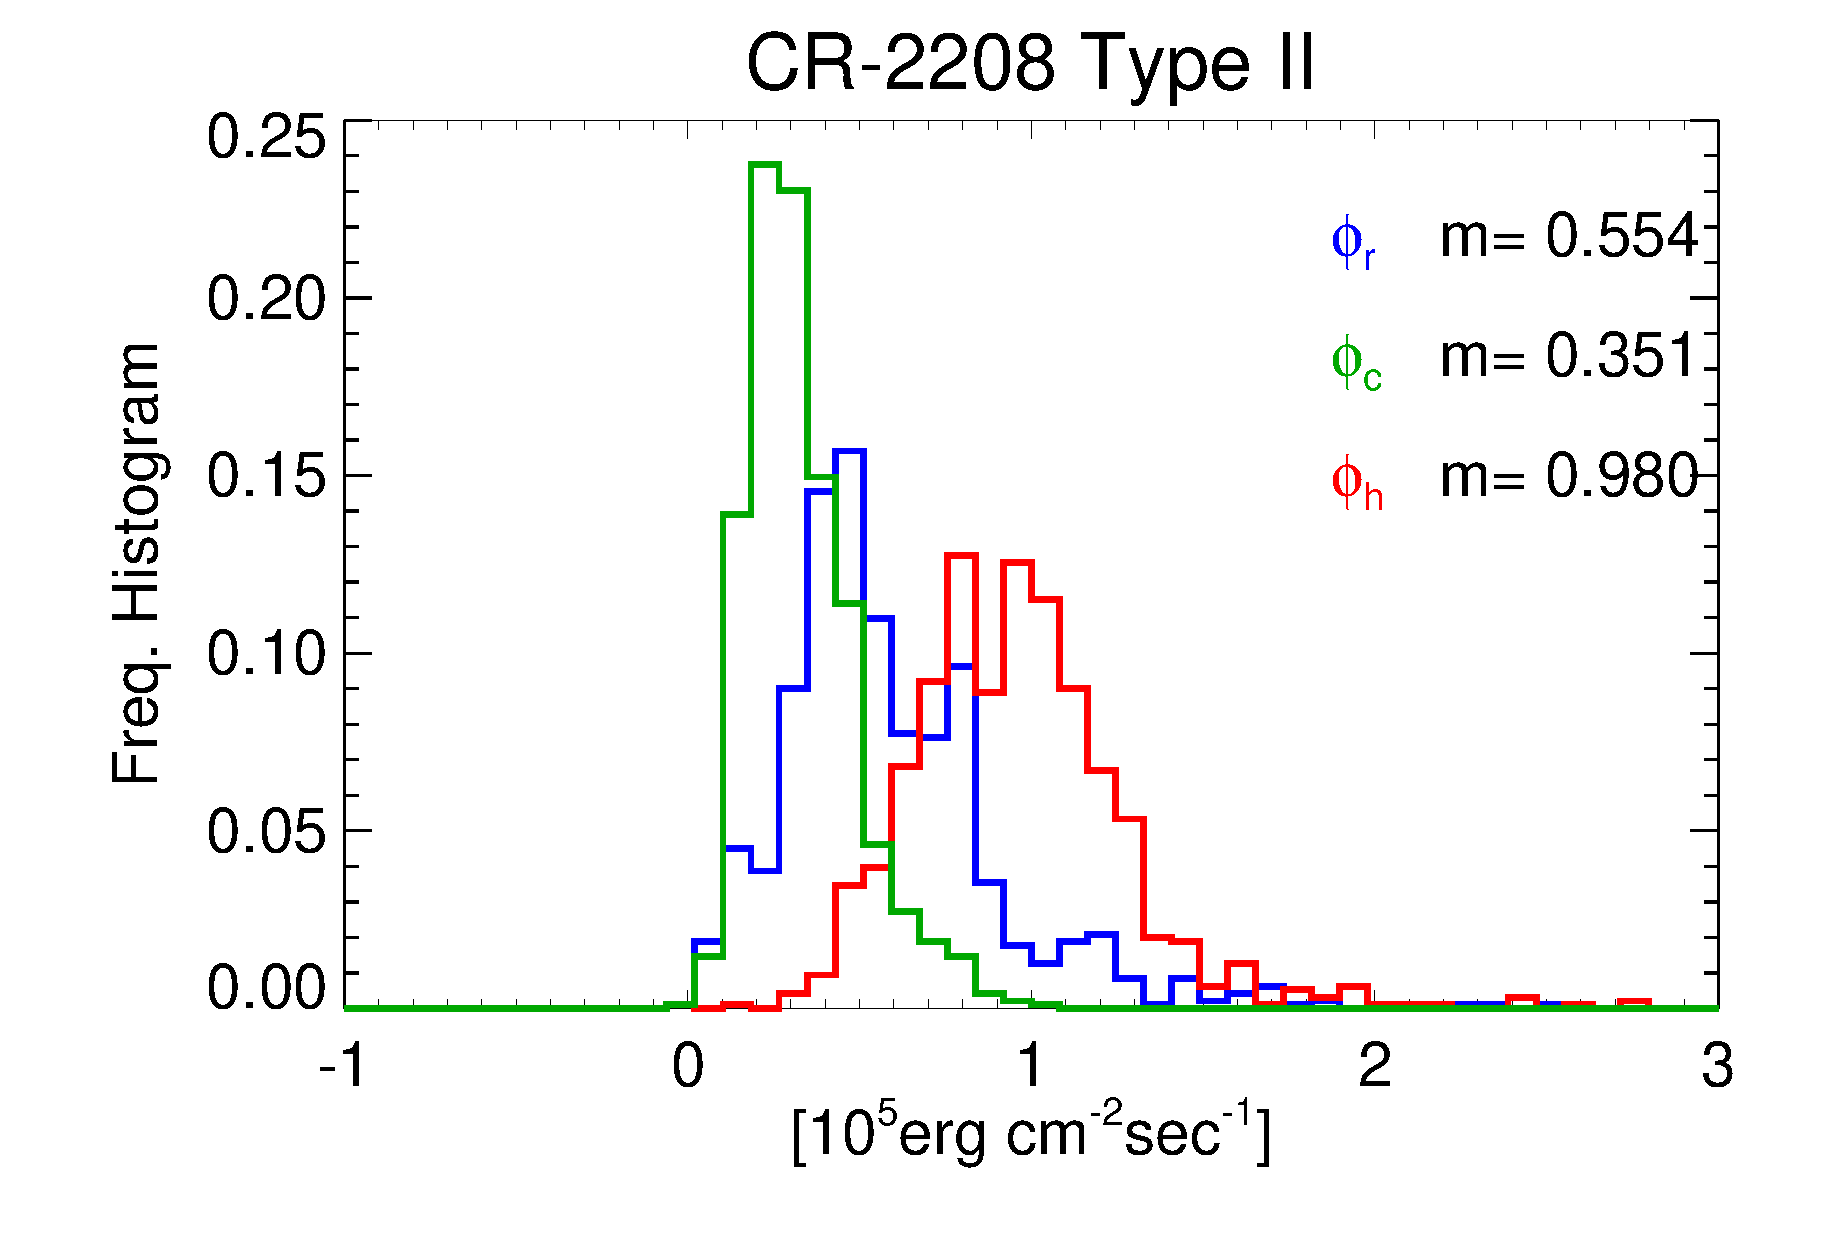
\includegraphics[width=0.495\textwidth,clip=]{figs/histocr2208_cgenergia.eps}
\caption{Statistical results of the loop integrated energy flux quantities $\phi_r,\phi_c,$ and $\phi_h$ in colours blu, red and green, respectively for CR-2082 (left) and CR-2208 (right). From top to left the type 0, 1 and 2 field of lines defined in Section \ref{trace}. }
\label{energia_demt}
\end{center}
\end{figure} 




\subsection{Tomography and Models}\label{awsom_res} 

\temp{Parrafo introductorio?}


As an example of the AWSoM results, Figures \ref{carmaps_awsom_2082} and \ref{carmaps_awsom_2208} shows the latitude-longitude maps for $\Ne$ and $T_e$ modeled for CR-2082 and CR-2208 at $r=1.025, 1.065$ and $1.105\,\mrsun$. The black curve denotes the open-close boundary.



A visual inspection of the AWSoM results shows that both reconstruction are very axysimmetric for $\Ne$ and $T_e$ as well. The closed region is denser and hotter than the open region. The density and temperature gradients are maximum in the open-close boundary. The open field regions in low latitudes maintain thermodynamic values associated with open regions. CR-2208 shows a well reconstruction of the AR around latitude $+10\mdeg$ and longitude $300\mdeg$ and a slight temperature difference between the poles \temp{estoy asumiento que es una AR}. 
In both rotations the open-closed boundaries derived from the respective AWSoM model match the shape of the contour levels of the tomographic maps of both the electron density and the electron mean temperature.


\begin{figure}[h!]
\begin{center}
\includegraphics[width=0.495\textwidth]{figs/map_Ne_awsom_2082_185_short_1025_Rsun.pdf}
\includegraphics[width=0.495\textwidth]{figs/map_Te_awsom_2082_185_short_1025_Rsun.pdf}
\includegraphics[width=0.495\textwidth]{figs/map_Ne_awsom_2082_185_short_1065_Rsun.pdf}
\includegraphics[width=0.495\textwidth]{figs/map_Te_awsom_2082_185_short_1065_Rsun.pdf}
\includegraphics[width=0.495\textwidth]{figs/map_Ne_awsom_2082_185_short_1105_Rsun.pdf}
\includegraphics[width=0.495\textwidth]{figs/map_Te_awsom_2082_185_short_1105_Rsun.pdf}
\caption{Carrington maps of density (left panels) and temperature (right panels) obtained with AWSoM model for the same three heights shown in Figure \ref{carmaps_demt_2082}.}
\label{carmaps_awsom_2082}
\end{center}
\end{figure}

\begin{figure}[h!]
\begin{center}
\includegraphics[width=0.495\textwidth]{figs/map_Ne_awsom_2208_185_short_1025_Rsun.pdf}
\includegraphics[width=0.495\textwidth]{figs/map_Te_awsom_2208_185_short_1025_Rsun.pdf}
\includegraphics[width=0.495\textwidth]{figs/map_Ne_awsom_2208_185_short_1065_Rsun.pdf}
\includegraphics[width=0.495\textwidth]{figs/map_Te_awsom_2208_185_short_1065_Rsun.pdf}
\includegraphics[width=0.495\textwidth]{figs/map_Ne_awsom_2208_185_short_1105_Rsun.pdf}
\includegraphics[width=0.495\textwidth]{figs/map_Te_awsom_2208_185_short_1105_Rsun.pdf}
\caption{Same as Figure \ref{carmaps_awsom_2208} for CR-2208.}
\label{carmaps_awsom_2208}
\end{center}
\end{figure}

\temp{Se presentan los midpoints para awsom que lucen mas rellenos xq no hay down loops y todo es super suave.}

In the same way as in Section \ref{demt_res}, the model results were traced along the magnetic lines obtained with it. This allowed to obtain $\Ne(r)$ and $T_e(r)$ along the magnetic lines and fit them to the Equations \ref{Nfit} and \ref{Tfit}.

Due to the inability of the model to reproduce down legs, in this section we only used lines type 1, 2 and 3 and only were selected those that meet the chi square hypothesis test.

Figure \ref{rpoint_awsom} shows the latitudinal-longitudinal location of the selected lines at $1.105\,\mrsun$ for both rotations. In blue the type 1 lines, populating mostly the entire streamer. In red the type 2 lines, populating the edge that assemble the envelope around the streamer, and in green dots the type 3 lines, populating the coronal holes.

The fact that Figure \ref{rpoint_awsom} looks much fuller than Figure \ref{rpoint_demt} is because giving the model smoother results, fewer fitted lines are filtered.

The reader may notice that these structures are the same as those in Figure \ref{rpoint_demt} but more filled, this is because the same magnetic result was used to trace both DEMT and AWSoM results.


\begin{figure}[h!]
\begin{center}
%\includegraphics[width=0.495\textwidth,clip=]{Highpoint_2082_demt_paper_Rpoint-map.eps}
\includegraphics[width=0.495\textwidth,clip=]{figs/Highpoint_2082_awsom_paper_cr2082_up_Rpoint-map.eps}
%\includegraphics[width=0.495\textwidth,clip=]{Highpoint_2208_demt_paper_Rpoint-map.eps}
\includegraphics[width=0.495\textwidth,clip=]{figs/Highpoint_2208_awsom_paper_cr2208_up_Rpoint-map.eps}
\caption{Same as Figure \ref{rpoint_demt}, using the density and temperature of AWSoM model to classify legs in type 1, 2 and 3.}
\label{rpoint_awsom}
\end{center}
\end{figure} 


To highlight the latitudinal structures observed in Figures \ref{carmaps_demt_2082} and \ref{carmaps_awsom_2082} for CR-2082 as well as Figures \ref{carmaps_demt_2208} and \ref{carmaps_awsom_2208} for CR-2208, Figure \ref{perf_lat} shows for both rotations the latitudinal variation  of both the electron density and the electron mean temperature at the height $r=1.105\,\mrsun$, averaged over all longitudes (excluding the AR). DEMT results are shown in blue lines while AWSoM results in red. While the temperature shows a maximum in each hemisphere, the density has a simpler behavior, with higher values in the low-latitudes of the streamer and a nearly monotonic decrease towards larger latitudes. The vertical black lines denotes the average of the open-close boundary in both hemispheres to each rotation.

\diego{Me gustaria hacer un comentario de cierre para esta figura que refiera las Figuras 3 y 9, como la linea de abajo, y que conecte con los histogramas que vienen a continuacion. Si no queda bien, hay que mover esta figura entre la actual figura 8 y 9.}

This longitude-averaged behaviors match well with the physical locations of the legs shown in Figures \ref{rpoint_awsom} and \ref{rpoint_demt}.

\diego{
*awsom da valores mas altos en los polos\\
*Parece haber una buena coincidencia en CR2082 en Te yen CR2208 en Ne.\\
*En CR2082 en Ne demt es 20 \% mas grande que awsom en la zona cerrada.\\
*En cr2208 en Te, en la zona polar awsom es 30\% mas grande y awsom es 25\% mas grande en la region cerrada.
}

\begin{figure}[h!]
\begin{center}
\includegraphics[width=0.495\textwidth]{figs/Perfil_Ne_demt_awsom_2082_1105.eps}
\includegraphics[width=0.495\textwidth]{figs/Perfil_Ne_demt_awsom_2208_1105.eps}
\includegraphics[width=0.495\textwidth]{figs/Perfil_Te_demt_awsom_2082_1105.eps}
\includegraphics[width=0.495\textwidth]{figs/Perfil_Te_demt_awsom_2208_1105.eps}
\caption{Longitude-averaged electron density (top) and temperature (bottom) for DEMT (blue) and AWSoM (red) results at $1.105\,\mrsun$. The left (right) panels correspond to CR-2082 (CR2208). The vertical black line indicates the longitude-averaged latitudes of the open/close magnetic boundary.}
\label{perf_lat}
\end{center}
\end{figure}

To summarize the comparison between both results during both rotations at full height, it is shown in Figure \ref{perfiles_promedio} the average fits of $\Ne(r)$ and $T_e(r)$ for every type of legs.

\diego{Explicar lo que se observa:
- Ne 1.65 awsom menor que la de demt en CR2082 y mayor que la de CR2208 y debido a que decaen esponencialmente, el hecho que tiendan a valores similares conforme aumenta la altura implica escalas de altura similares. \\
- Las temperaturas a 1.065 difieren en ambas rotaciones y en todas las regiones/tipos de lineas siendo siempre menor la de awsom, sin embargo las pendientes son similares en todas la regiones. Excepto que los gradientes de cr2208 en CH son mayores demt consistente con la fig de grad de temp, me preg si esto es por AIA.}



\begin{figure}[h!]
\begin{center}
\includegraphics[width=0.495\textwidth,clip=]{figs/perfil_paper_ne_cr2082_up_short.eps}
\includegraphics[width=0.495\textwidth,clip=]{figs/perfil_paper_te_cr2082_up_short.eps}
\includegraphics[width=0.495\textwidth,clip=]{figs/perfil_paper_ne_cr2208_up_short.eps}
\includegraphics[width=0.495\textwidth,clip=]{figs/perfil_paper_te_cr2208_up_short.eps}
\caption{Average fits of $\Ne(r)$ and $T_e(r)$ for legs of type I (blue), type II (red) and type III (green) for CR-2082 (top panel) and CR-2208 (bottom panel) using DEMT (solid) and AWSoM (dashed) results.}
\label{perfiles_promedio}
\end{center}
\end{figure} 

As way of example, Figure \ref{histos_2082} and \ref{histos_2208} shows the statistical results of both rotations for the three types of field lines traced with DEMT (blue) and AWSoM results (red). From left to right the panels show the statistical distribution of $\NCB$, $\lN$ and $\aTm$. For all types of lines, Table \ref{tabla_comp} summarizes the median value of the statidtical distribution of each physical quantity derived from the analysis. The DEMT quantities are expressed as absoulte values, while for ASWSoM they are informed relative to the corresponding result for DEMT.

\diego{comentar lo que se desprende de los graficos y la tabla.}

\begin{figure}[h!]
\begin{center}
\includegraphics[width=0.31\textwidth,clip=]{figs/histo_2082_demt_awsom_streamer_up_ne_1055.eps}
\includegraphics[width=0.31\textwidth,clip=]{figs/histo_2082_demt_awsom_streamer_up_lambda_n.eps}
\includegraphics[width=0.31\textwidth,clip=]{figs/histo_2082_demt_awsom_streamer_up_Tm.eps}
\includegraphics[width=0.31\textwidth,clip=]{figs/histo_2082_demt_awsom_bound_up_ne_1055.eps}
\includegraphics[width=0.31\textwidth,clip=]{figs/histo_2082_demt_awsom_bound_up_lambda_n.eps}
\includegraphics[width=0.31\textwidth,clip=]{figs/histo_2082_demt_awsom_bound_up_Tm.eps}
\includegraphics[width=0.31\textwidth,clip=]{figs/histo_2082_demt_awsom_CH_up_ne_1055.eps}
\includegraphics[width=0.31\textwidth,clip=]{figs/histo_2082_demt_awsom_CH_up_lambda_n.eps}
\includegraphics[width=0.31\textwidth,clip=]{figs/histo_2082_demt_awsom_CH_up_Tm.eps}
\caption{Comparative statistical distributions for CR-2082 between DEMT (blue) and AWSoM (red). From left to right: the coronal base electron density $\Ne(r=1.055\,\mrsun)$, the electron density scale height $\lN$ and the average $\aTm$ along the four types of legs considered in Section \ref{trace}. In each panel the median ($m$) is indicated.}
\label{histos_2082}
\end{center}
\end{figure} 


\begin{table}
\begin{tabular}{l r@{.}l@{\hskip 0.05in} r@{\hskip 0.01in} r@{.}l  r@{.}l@{\hskip 0.05in} r@{\hskip 0.01in} r@{.}l r@{.}l@{\hskip 0.05in} r@{\hskip 0.01in} r@{.}l }
% r@{.}l@{\hskip 0.05in} r@{\hskip 0.01in} r@{.}l@{\hskip 0.01in} l}
\hline
Type    & \multicolumn{5}{c}{$\med(\NCB)$}             & \multicolumn{5}{c}{$\med(\lN)$} & \multicolumn{5}{c}{$\med(\avgTe)$} \\
       & \multicolumn{5}{c}{$[10^8\,{\rm cm}^{-3}]$}  & \multicolumn{5}{c}{$[{\rm 10}^{-2}\,\mrsun]$} & \multicolumn{5}{c}{$[\MK]$} \\
\hline
CR-2082\\
1  & 0&84 &(\Mi&14&4\%)  &   8&3 &(\Mi&~2&5\%) &   1&30 &(\Mi&10&8\%) \\
2  & 0&74 &(\Mi&21&9\%)  &   8&9 &(\Pl&~1&0\%) &   1&33 &(\Mi&~4&5\%) \\
3  & 0&82 &(\Mi&17&9\%)  &   7&7 &(\Mi&~8&9\%) &   0&98 &(\Mi&~9&5\%) \\
\hline          
CR-2208\\
1  & 0&74 &(\Pl&~6&4\%)  &   9&8 &(\Mi&~7&1\%) &   1&55 &(\Mi&12&3\%) \\
2  & 0&62 &(\Pl&~8&2\%)  &  11&6 &(\Mi&17&2\%) &   1&55 &(\Mi&~9&7\%) \\
3  & 0&42 &(\Mi&~4&8\%)  &   8&6 &(\Mi&~8&4\%) &   1&04 &(\Mi&~9&7\%) \\
\end{tabular}
\caption{Median value (indicated as ``Md'') of the statistical distribution of $\NCB$, $\lN$, and $\aTm$ for each coronal type of lines defined in Section \ref{trace}. FDEMT values are expressed in absolute terms, while for AWSoM they are informed as a percentual variation relative to the DEMT value.}
\label{tabla_comp}
\end{table}



%For both rotations, all field lines that meet the criteria listed in Section \ref{trace} were separated into the coronal {regions described in Section \ref{regions} and summarized in Table \ref{tabregions}}. For each field line, the data points of electron density and electron mean temperature versus height were fitted to the functions given by Equations 5 and 6 of Section \ref{trace}. As a result, the footpoint electron density $N_0$ and scale height $\lN$ were computed for each field line, as well as the temperature gradient $a=\textrm{d}\Tm/\textrm{d}r$, and the height-averaged (along the loop) electron mean temperature $\aTm$. As the DEMT technique studies only coronal conditions, \textit{i.e.} above height $r\approx 1.025\,\mrsun$, the exponential fit to the electron density data versus height was used to compute the {coronal base electron density} here defined as $\NCB\equiv \Ne(r=1.025\,\mrsun)$. Also, for each field line the coronal base magnetic field strength $B_{\rm CB}\equiv B(r=1.025\,\mrsun)$ and its height-averaged value along the loop $\left<B\right>$ were also computed.

\begin{figure}[h!]
\begin{center}
\includegraphics[width=0.31\textwidth,clip=]{figs/histo_2208_demt_awsom_streamer_up_ne_1055.eps}
\includegraphics[width=0.31\textwidth,clip=]{figs/histo_2208_demt_awsom_streamer_up_lambda_n.eps}
\includegraphics[width=0.31\textwidth,clip=]{figs/histo_2208_demt_awsom_streamer_up_Tm.eps}\\
\includegraphics[width=0.31\textwidth,clip=]{figs/histo_2208_demt_awsom_bound_up_ne_1055.eps}
\includegraphics[width=0.31\textwidth,clip=]{figs/histo_2208_demt_awsom_bound_up_lambda_n.eps}
\includegraphics[width=0.31\textwidth,clip=]{figs/histo_2208_demt_awsom_bound_up_Tm.eps}\\
\includegraphics[width=0.31\textwidth,clip=]{figs/histo_2208_demt_awsom_CH_up_ne_1055.eps}
\includegraphics[width=0.31\textwidth,clip=]{figs/histo_2208_demt_awsom_CH_up_lambda_n.eps}
\includegraphics[width=0.31\textwidth,clip=]{figs/histo_2208_demt_awsom_CH_up_Tm.eps}
\caption{Same as Figure \ref{histos_2082} for CR-2208.}
\label{histos_2208}
\end{center}
\end{figure} 


%This plot (E) has never been shown before and I believe it is a very nice result. There are of course previous studies on this, but this would be the first time this is evaluated with tomography. It is not the terminal speed, but it already shows the fast/slow components. We can show this, or we can go for more. Diego can QUANTIFY the correlation by carefully mapping all open field lines at 6 Rsun down to the DEMT region. He needs to code a bit more to achieve this goal, but we believe it is worth. With that tool done Diego can explore other terminal values of quantities of the AWSoM model and the DEMT results below (expansion factor maybe?). This will be nice to do also for the July-2-2019 Eclipse rotation that we will analyze after this paper. 



Figure \ref{perf_lon_vr} show the longitude-averaged AWSoM radial wind speed $V_r$ at $6\,\mrsun$, where all field lines are open. The heliocentric current sheet (HCS) location is indicated by the minimum of the speed curve.\\
\diego{can we say something without having traced the lines?}

For each rotation, everything to the south of the HCS maps down to the southern open region in the Figures \ref{perf_lat}, and the same for the northern hemisphere, showing an anti-correlation between $\Ne$ at low heights and high $V_r$ at $6\,\mrsun$.

\diego{Voy a intentar jugar con las lineas tipo 3 aumentando su cota inferior de latitud para ver si los histogramas de temp media dejan de ser tan dispersos y se vuelven mas sub-1MK. }


\begin{figure}[h!]
\begin{center}
\includegraphics[width=0.495\textwidth]{figs/Perfil_Vr_2082_5995.eps}
\includegraphics[width=0.495\textwidth]{figs/Perfil_Vr_2208_5995.eps}
\caption{Longitude-averaged of radial wind speed at $6\,\mrsun$ given by AWSoM for both rotations.}
\label{perf_lon_vr}
\end{center}
\end{figure}



\section{Discussion}\label{discu} 

*Down loops, shiff y cranmer comentarios.




%% Figure 
%
% \begin{figure} 
% \centerline{\includegraphics[width=0.5\textwidth,clip=]{<fig.eps>}}
% \caption{}%\label{fig:?}
% \end{figure}



%% Table
%
% \begin{table}
% \caption{}%\label{tbl:?}
% \begin{tabular}{}     
% \hline
% \multicolumn{2}{c}{<>}
% <data>
% \hline
% \end{tabular}
% \end{table}
  

%%%%%%%%%%%%%%%%%%%%%%%%%%%%%%%%%%%%%%%%%%%%%%%%%%%%%%%%%%%%%%%%%%%%%%%%%%%
%% Appendix
%
% \appendix   



%%%%%%%%%%%%%%%%%%%%%%%%%%%%%%%%%%%%%%%%%%%%%%%%%%%%%%%%%%%%%%%%%%%%%%%%%%%
%% Acknowledgements
%
% \begin{acks}
%
% \end{acks}


%%% %%%%%%%%%%%%%%%%%%%%%%%%%%%%%%%%%%%%%%%%%%%%%%%%%%%%%%%%%%%
%% Bibliography
%
% Using BibTeX
%
\bibliographystyle{spr-mp-sola}
\bibliography{solphys_dglloveras}  
%
% Without BibTeX 
% \begin{thebibliography}{}
% \bibitem[\protect\citeauthoryear{Author}{Year}]{key}
%   <bibliographical entry>
%
% \bibitem[\protect\citeauthoryear{}{}]{}
%   
%  
% \end{thebibliography}

\end{article} 
\end{document}
